
We evaluate the performance of the proposed methodology for the task of human body pose correspondence estimation, as well as non-rigid alignment ``in-the-wild''. For further experimental results, please refer to the supplementary material.

%Results of quantitative and qualitative evaluations are reported.

\begin{figure}[t!]
    \centering
    \includegraphics[width=\columnwidth]{resources/Fig_Variance/final}
    \caption{Example of human pose annotation for left arm among 4 annotators. The large variance shows the difficulties of having consistent landmarks. Figure best viewed by zooming in.}
    \label{fig:variance}
\end{figure}

\begin{figure*}[!t]
    \newcommand{\fh}{0.24\columnwidth}
    \centering
    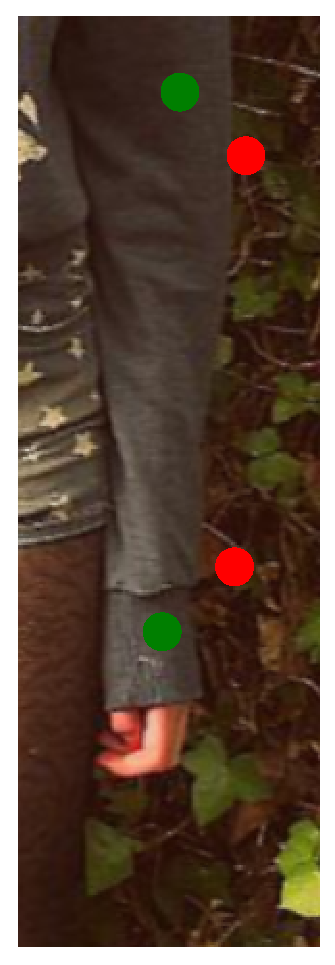
\includegraphics[height=\fh]{resources/Fixing/fix_1}
    \hfill
    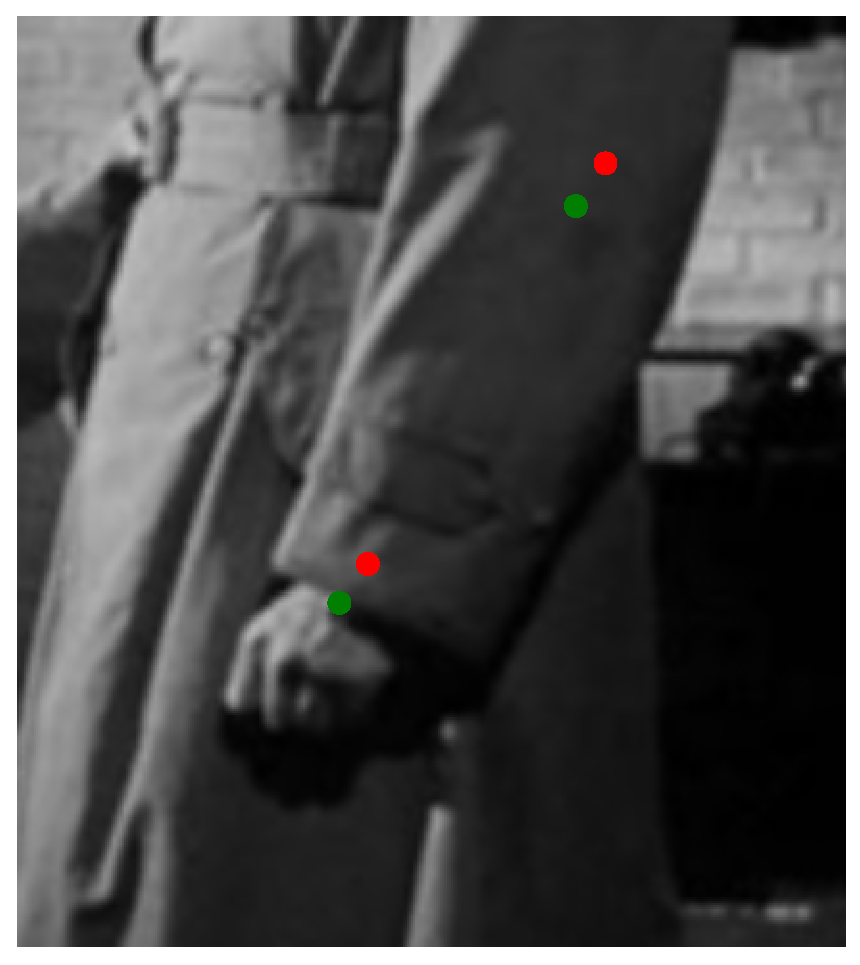
\includegraphics[height=\fh]{resources/Fixing/fix_2}
    \hfill
    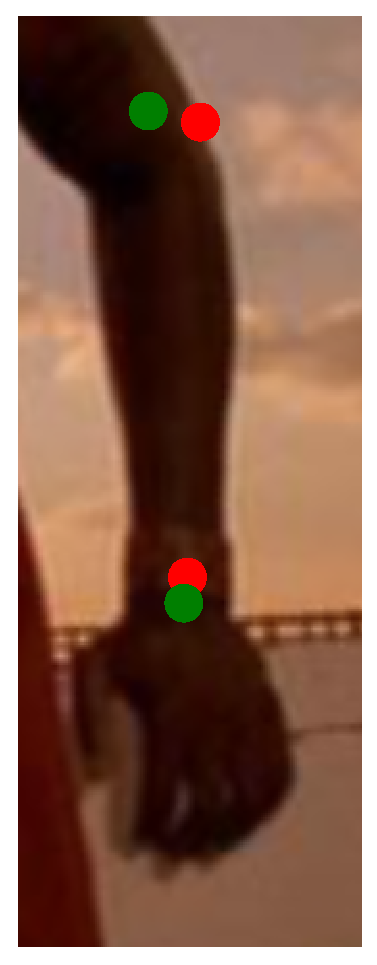
\includegraphics[height=\fh]{resources/Fixing/fix_3}
    \hfill
    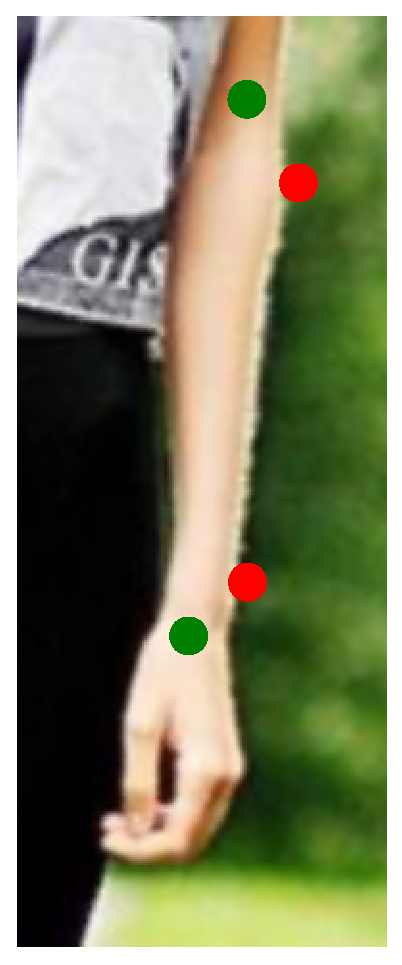
\includegraphics[height=\fh]{resources/Fixing/fix_5}
    \hfill
    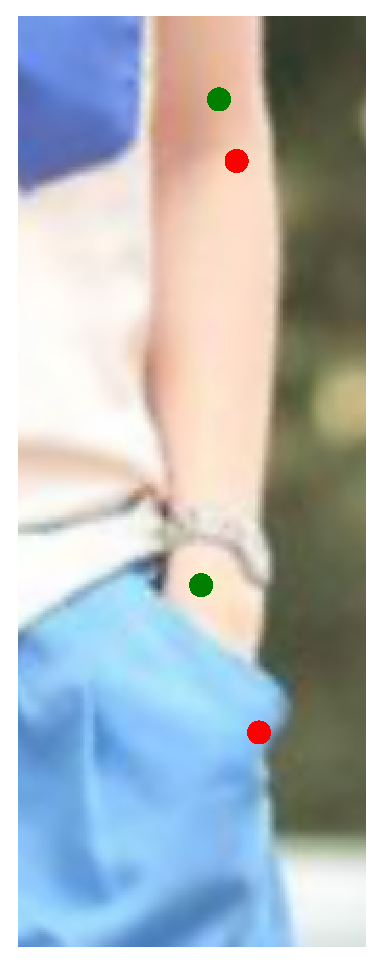
\includegraphics[height=\fh]{resources/Fixing/fix_6}
    \hfill
    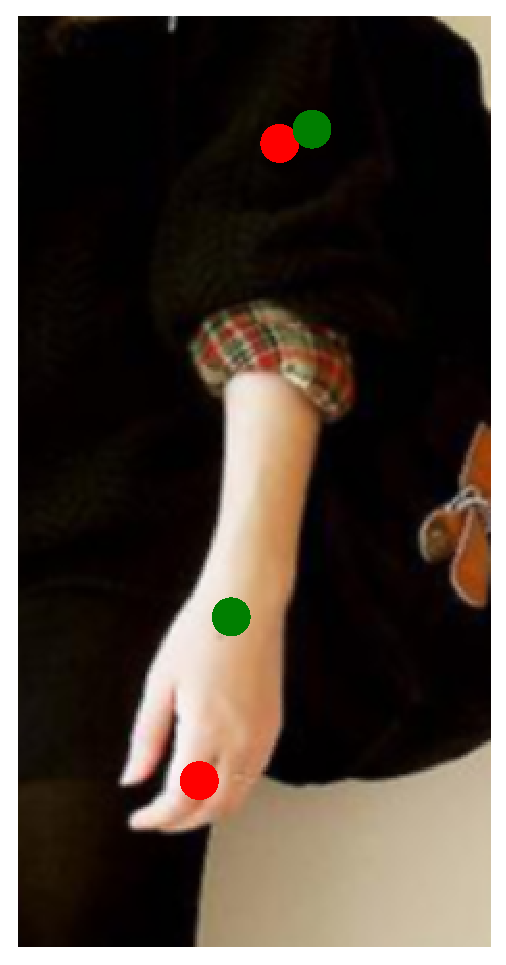
\includegraphics[height=\fh]{resources/Fixing/fix_7}
    \hfill
    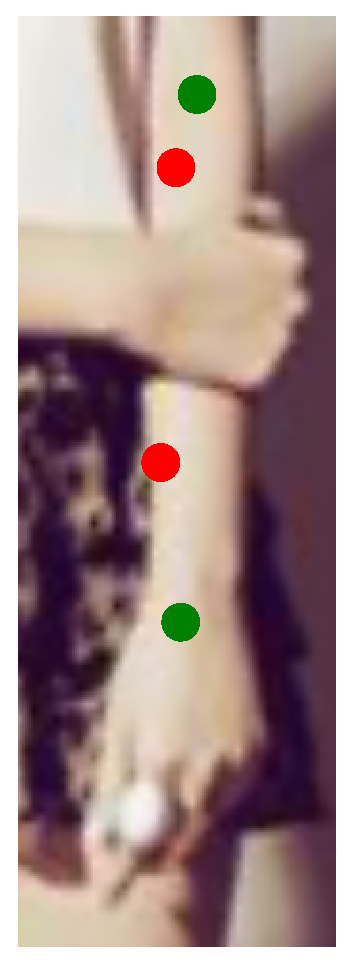
\includegraphics[height=\fh]{resources/Fixing/fix_8}
    \hfill
    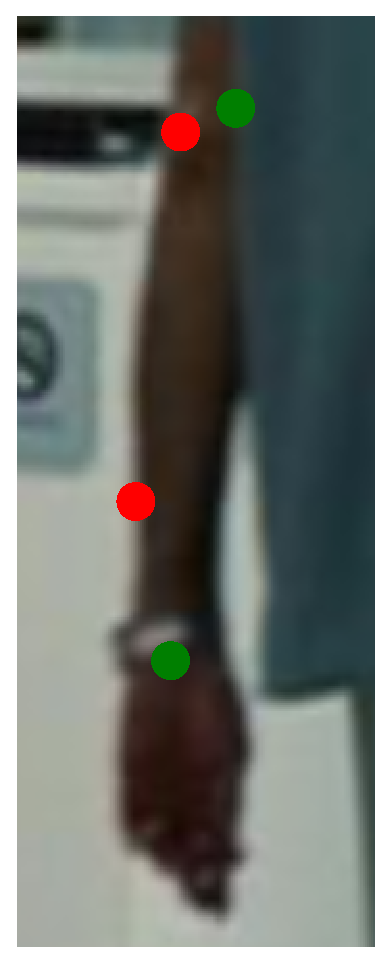
\includegraphics[height=\fh]{resources/Fixing/fix_9}
    \hfill
    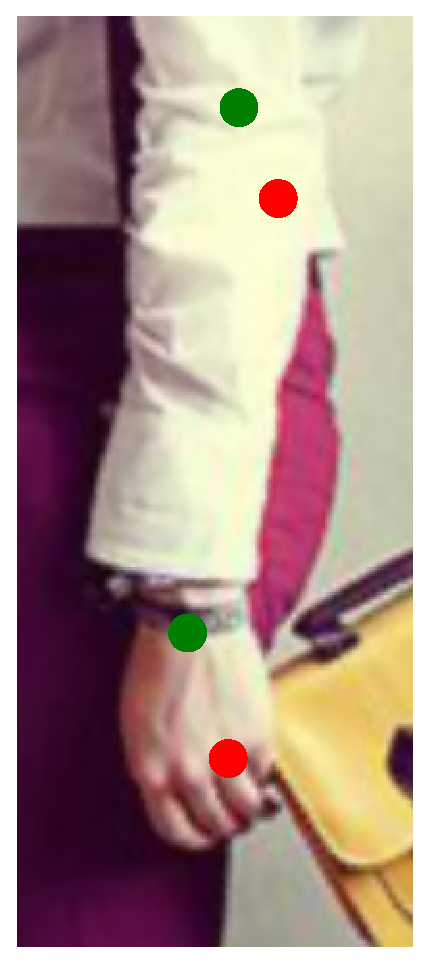
\includegraphics[height=\fh]{resources/Fixing/fix_10}
    \hfill
    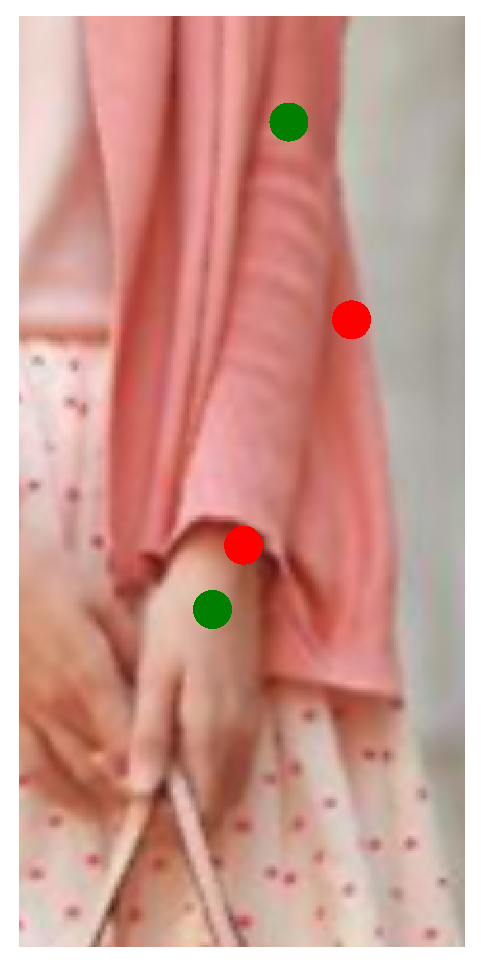
\includegraphics[height=\fh]{resources/Fixing/fix_20}
    \hfill
    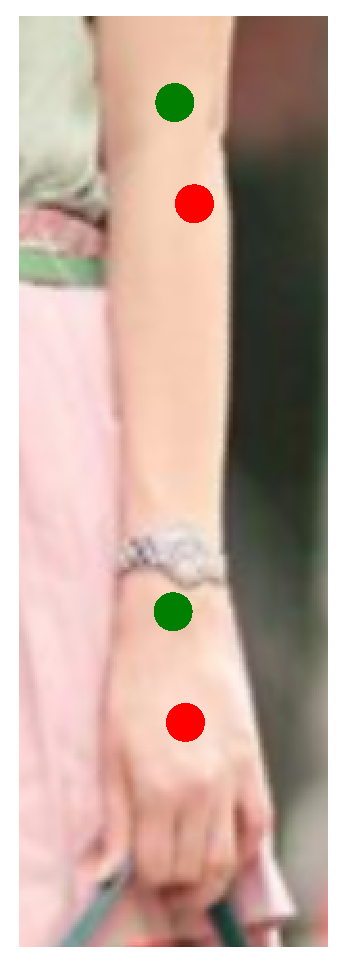
\includegraphics[height=\fh]{resources/Fixing/fix_12}
    \hfill
    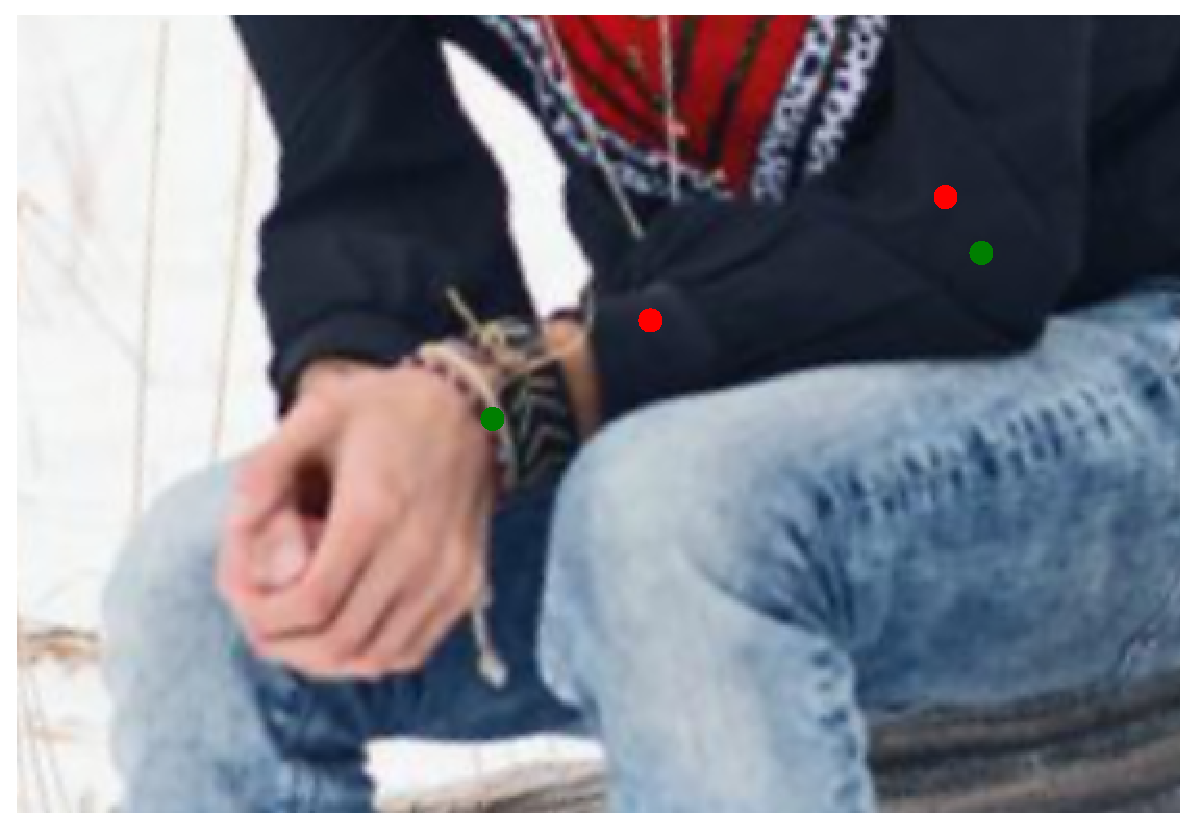
\includegraphics[height=\fh]{resources/Fixing/fix_13}
    \hfill
    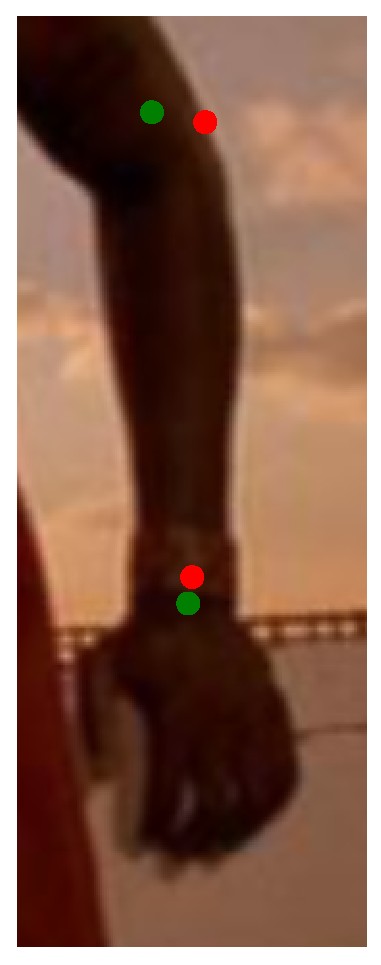
\includegraphics[height=\fh]{resources/Fixing/fix_14}
    \hfill
    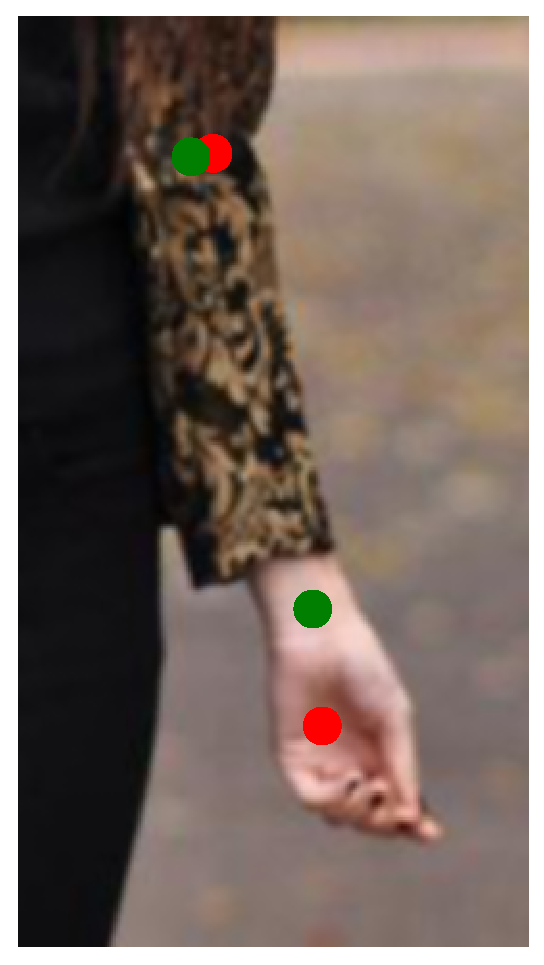
\includegraphics[height=\fh]{resources/Fixing/fix_15}
    \hfill
    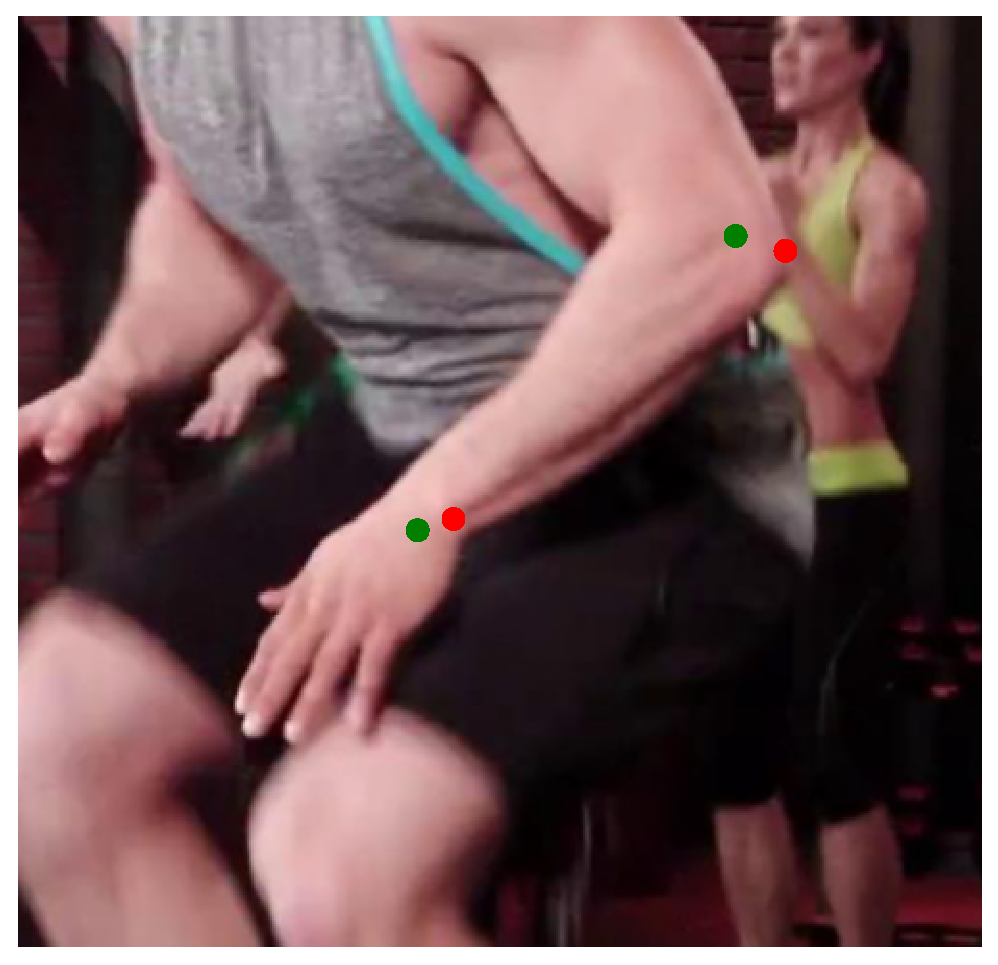
\includegraphics[height=\fh]{resources/Fixing/fix_17}
    \hfill
    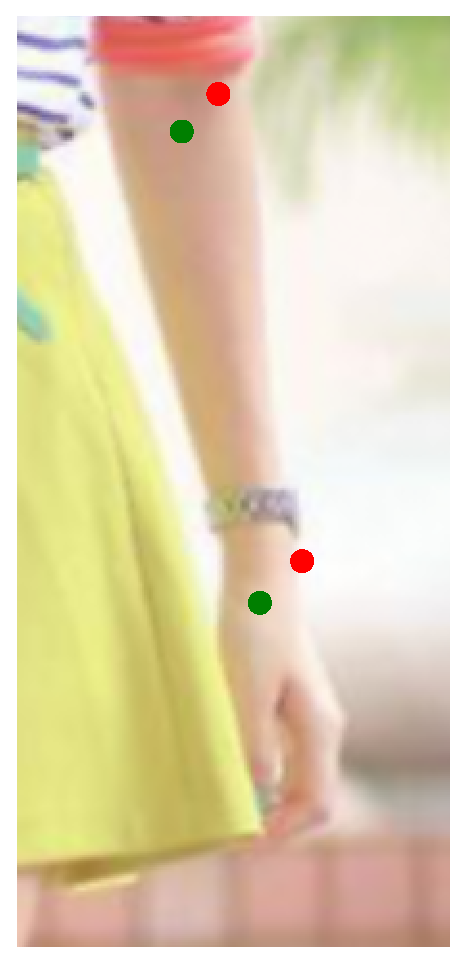
\includegraphics[height=\fh]{resources/Fixing/fix_18}
    \caption{Demonstration of annotation correction using our method for experiment \ref{exp:qualitative}. \emph{Red} dots refer to officially provided landmarks, and \emph{green} dots are corrected position.}
    \label{fig:qualitative}
\end{figure*}

\begin{figure*}[!t]
    \newcommand{\ofh}{0.24\columnwidth}
    \centering
    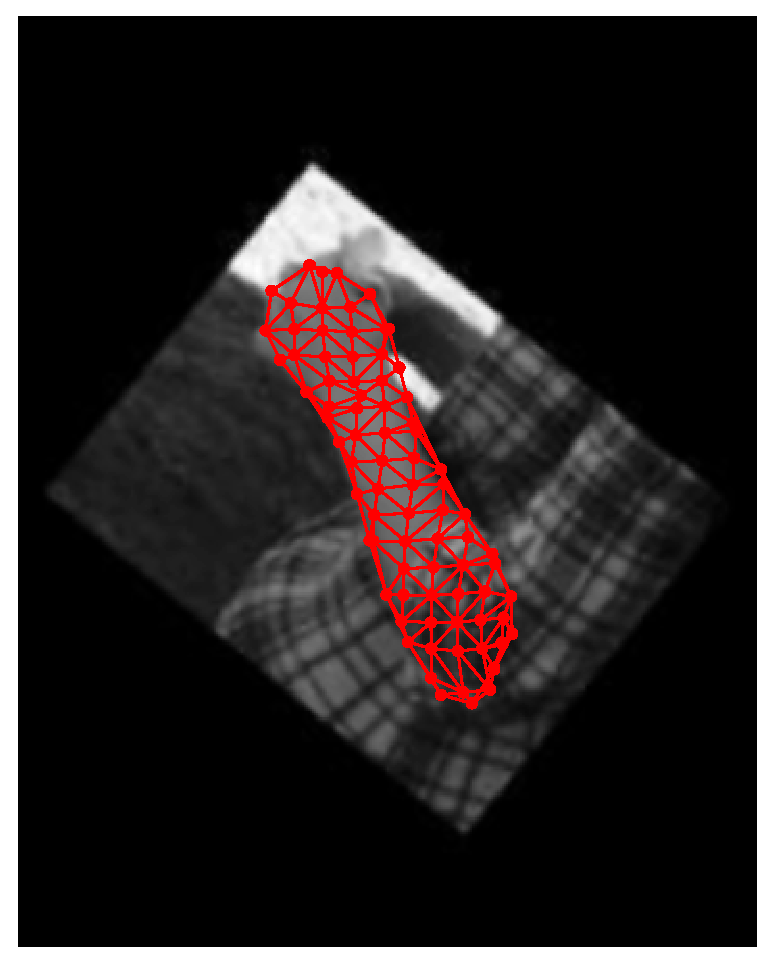
\includegraphics[height=\ofh]{resources/Fittings/20.eps}
    \hfill
    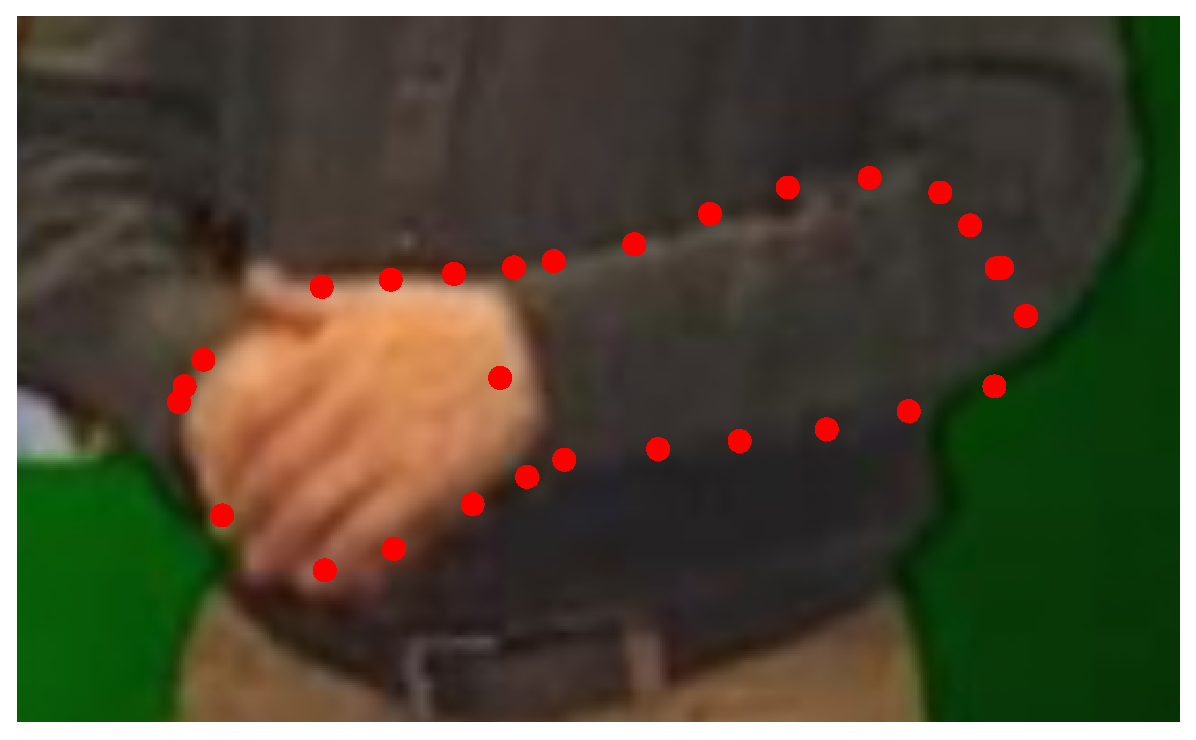
\includegraphics[height=\ofh]{resources/Fittings/3.eps}
    \hfill
    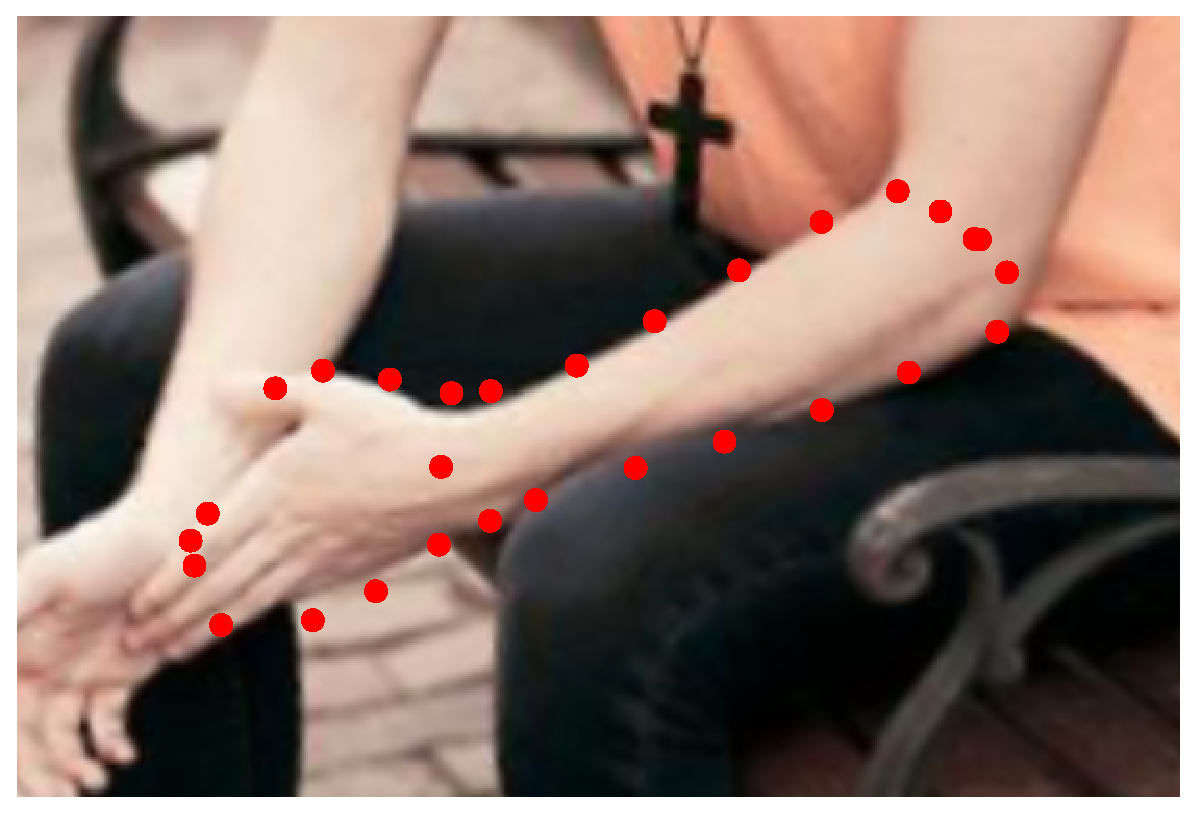
\includegraphics[height=\ofh]{resources/Fittings/19.eps}
    \hfill
    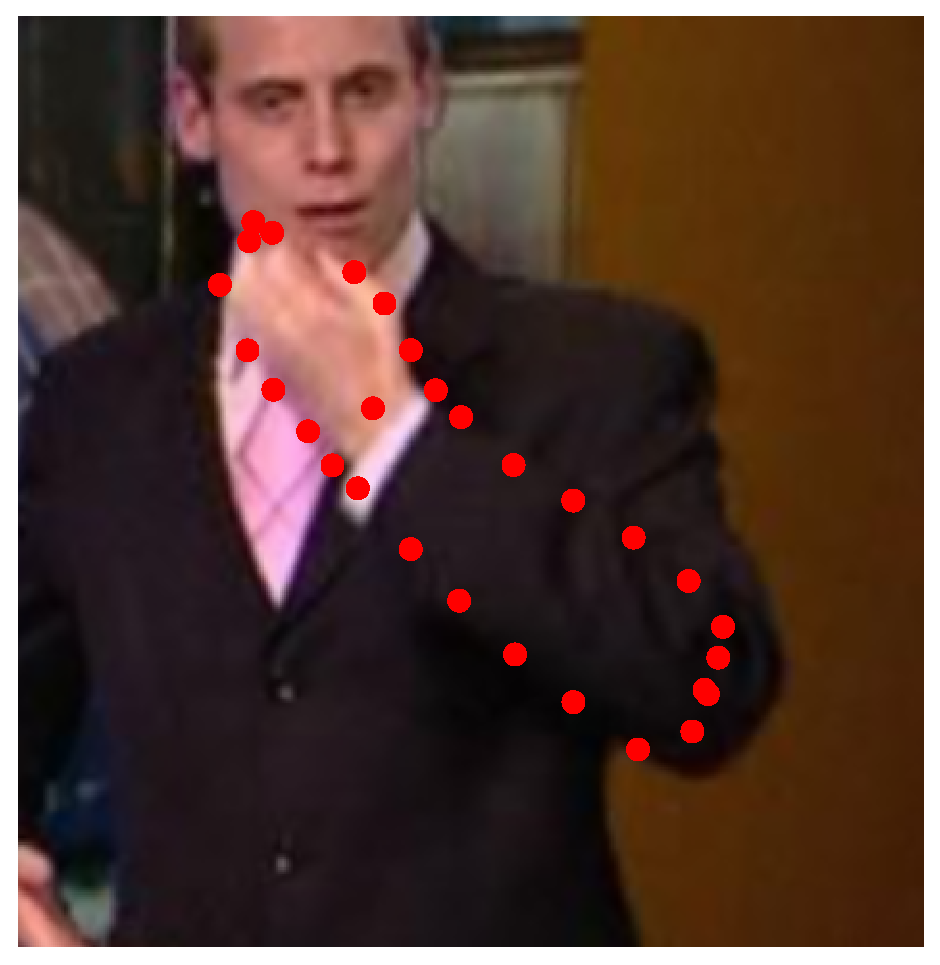
\includegraphics[height=\ofh]{resources/Fittings/4.eps}
    \hfill
    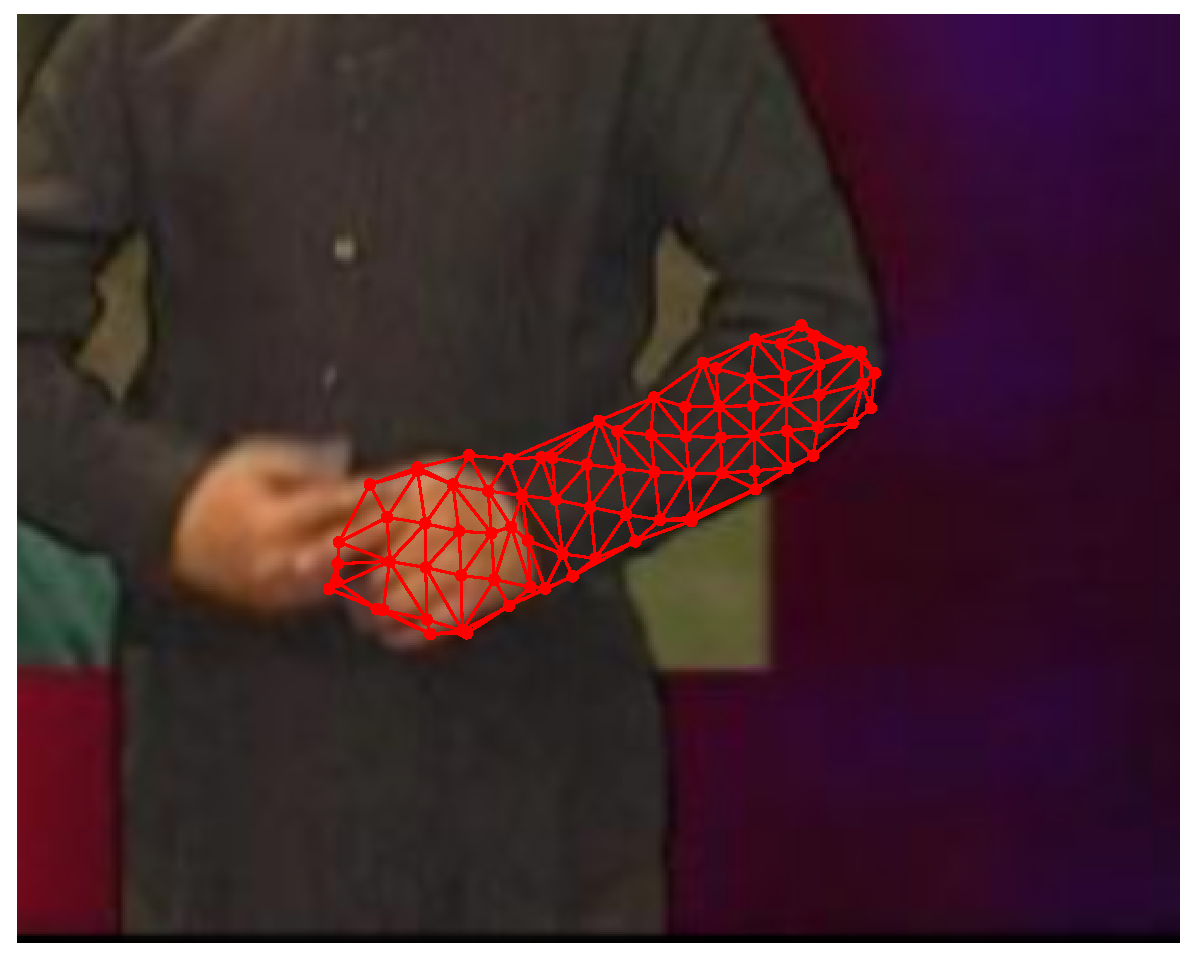
\includegraphics[height=\ofh]{resources/Fittings/6.eps}
    \hfill
    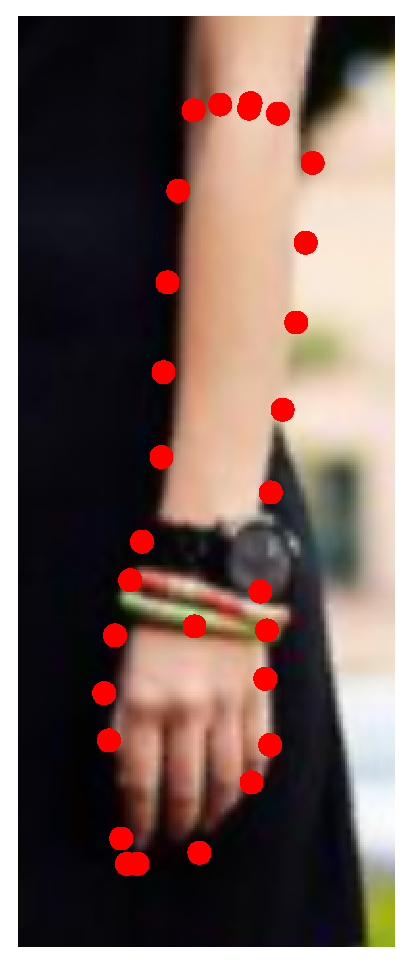
\includegraphics[height=\ofh]{resources/Fittings/15.eps}
    \hfill
    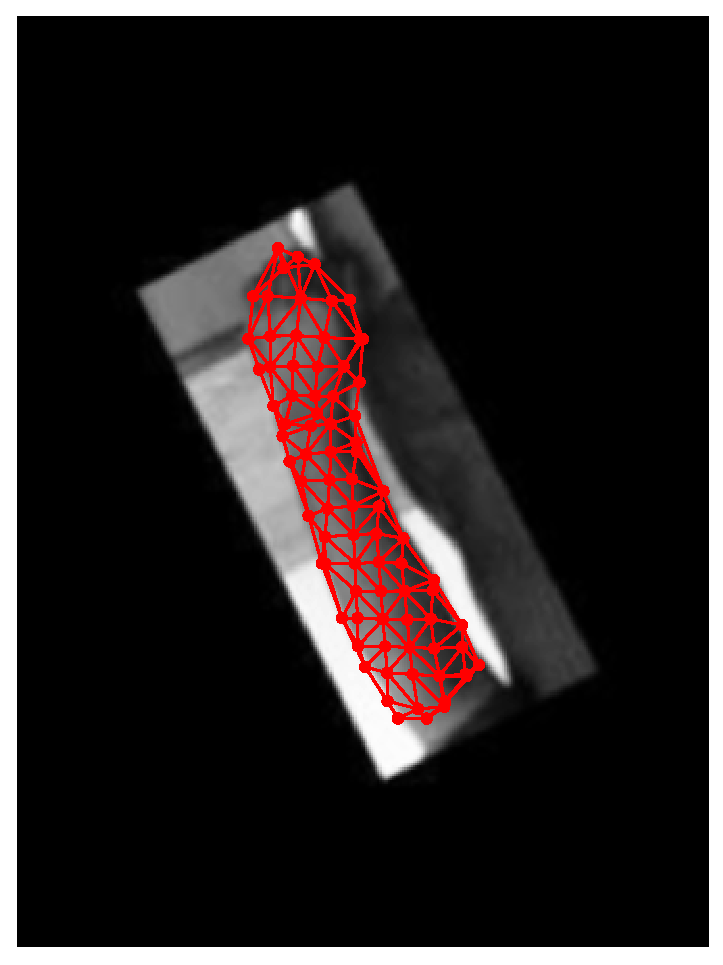
\includegraphics[height=\ofh]{resources/Fittings/7.eps}
    \hfill
    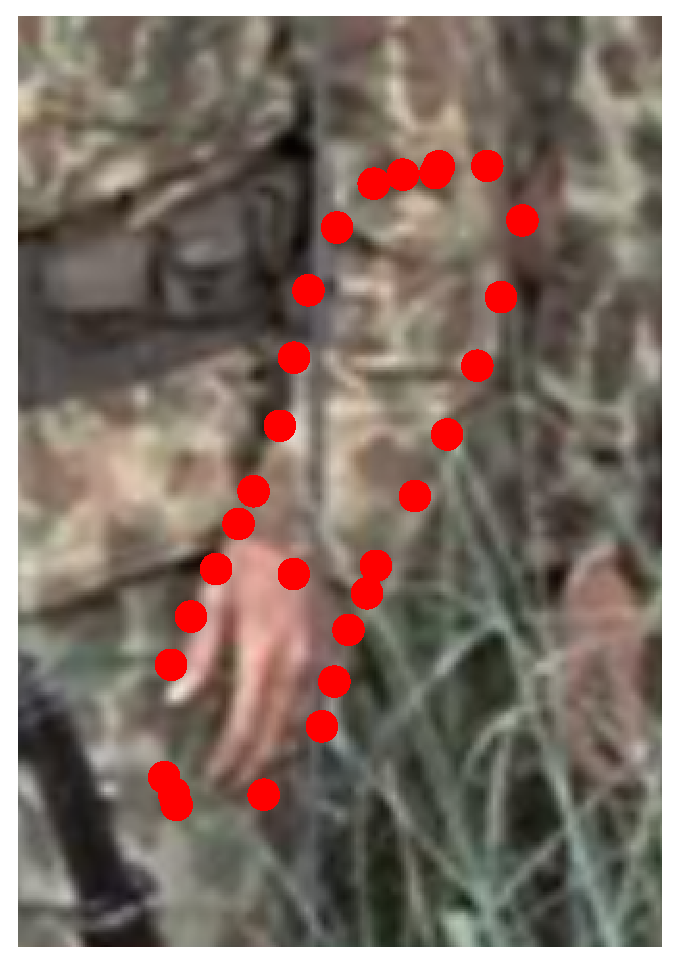
\includegraphics[height=\ofh]{resources/Fittings/8.eps}
    \hfill
    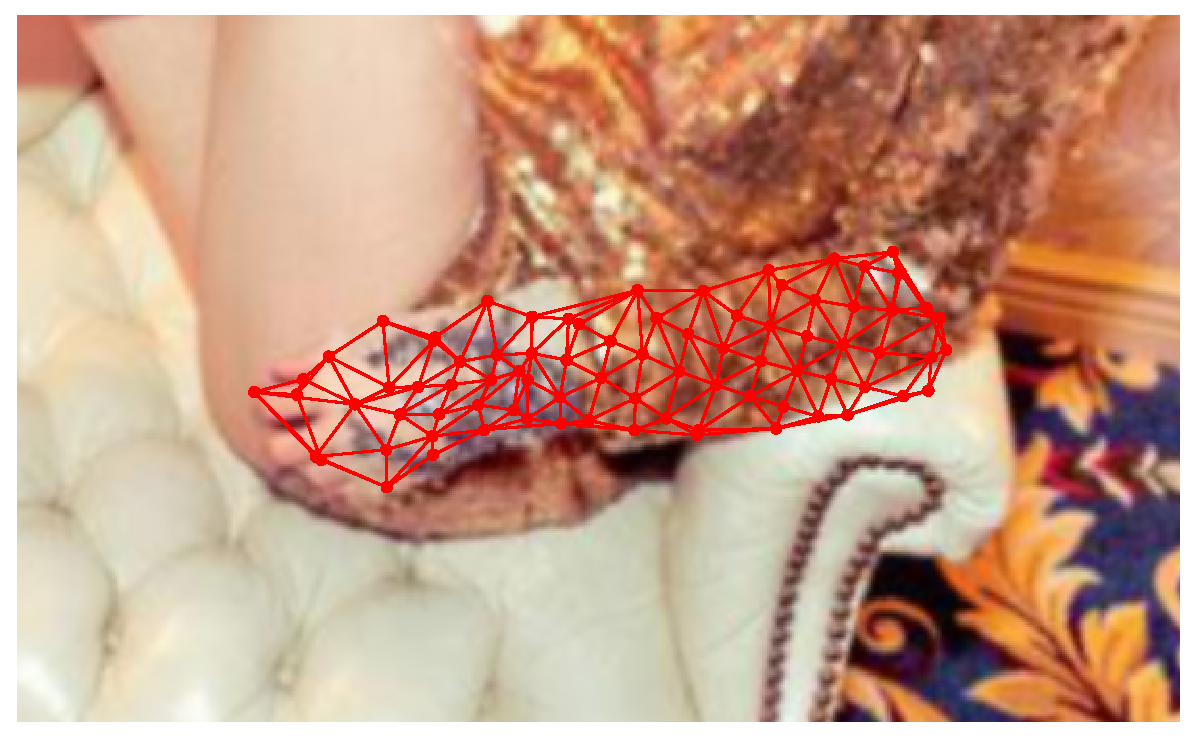
\includegraphics[height=\ofh]{resources/Fittings/13.eps}
    \hfill
    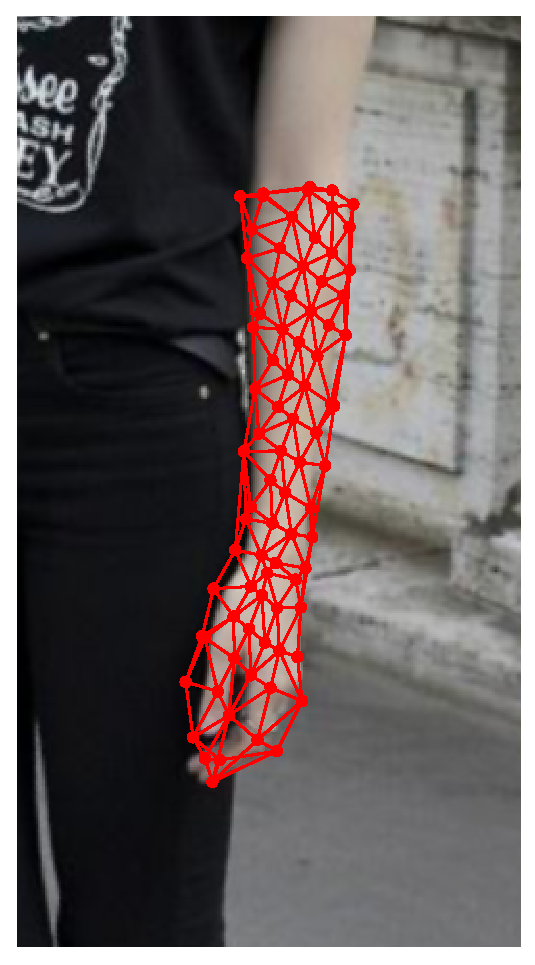
\includegraphics[height=\ofh]{resources/Fittings/17.eps}
    \\
    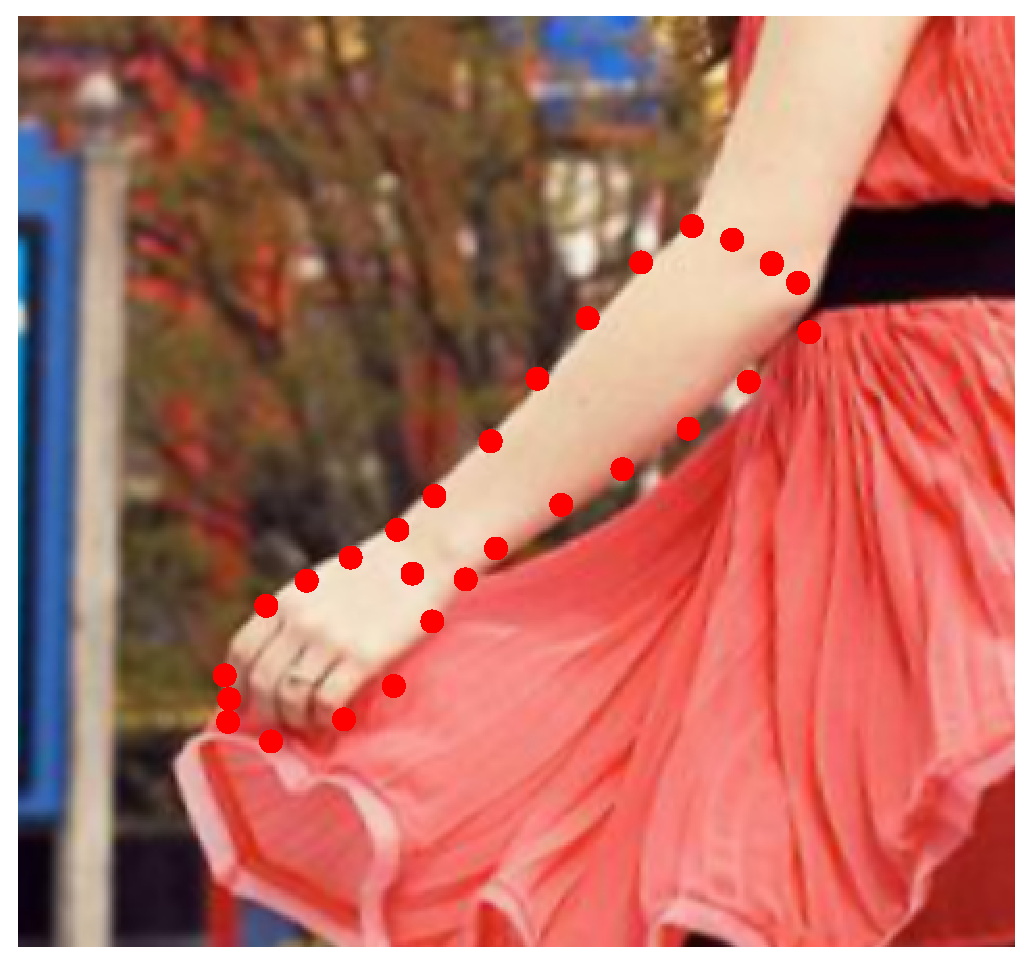
\includegraphics[height=\ofh]{resources/Fittings/21.eps}
    \hfill
    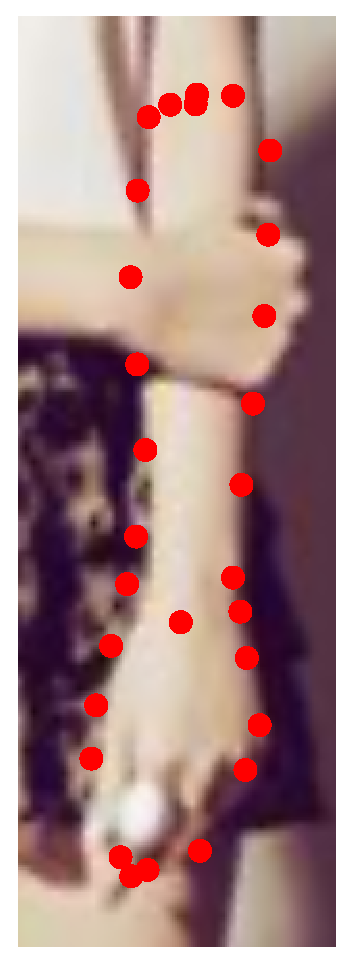
\includegraphics[height=\ofh]{resources/Fittings/23.eps}
    \hfill
    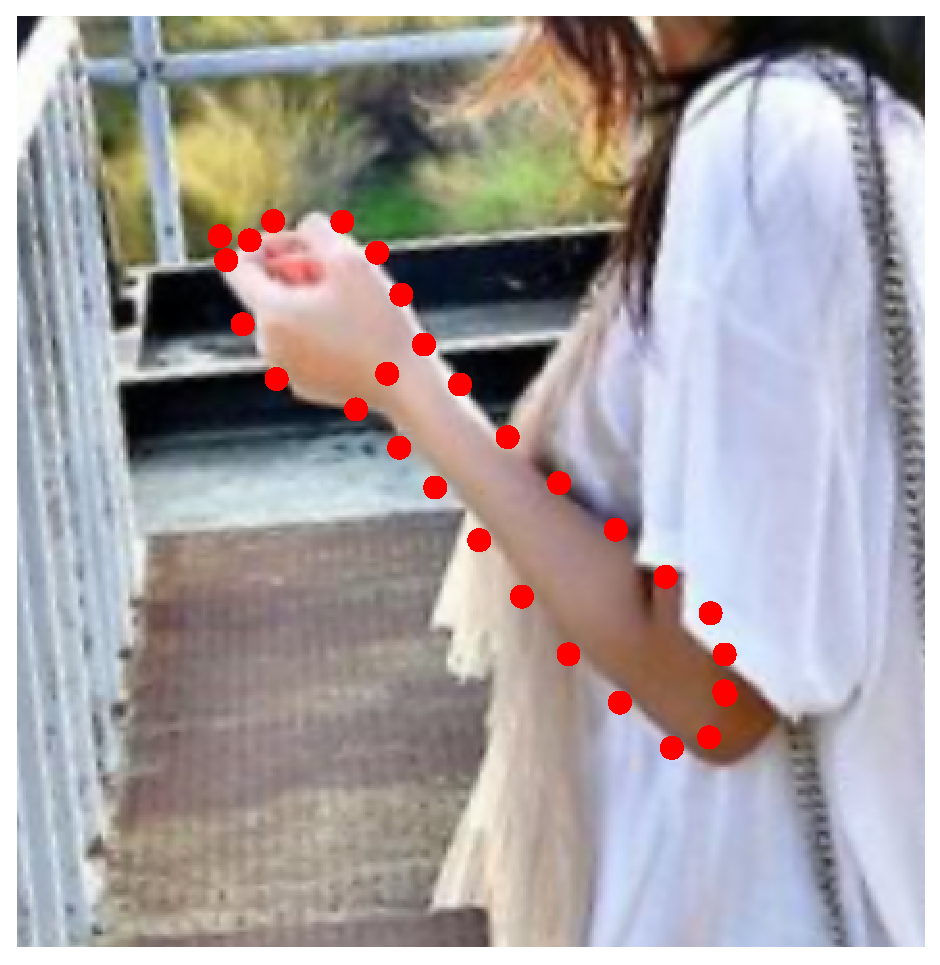
\includegraphics[height=\ofh]{resources/Fittings/25.eps}
    \hfill
    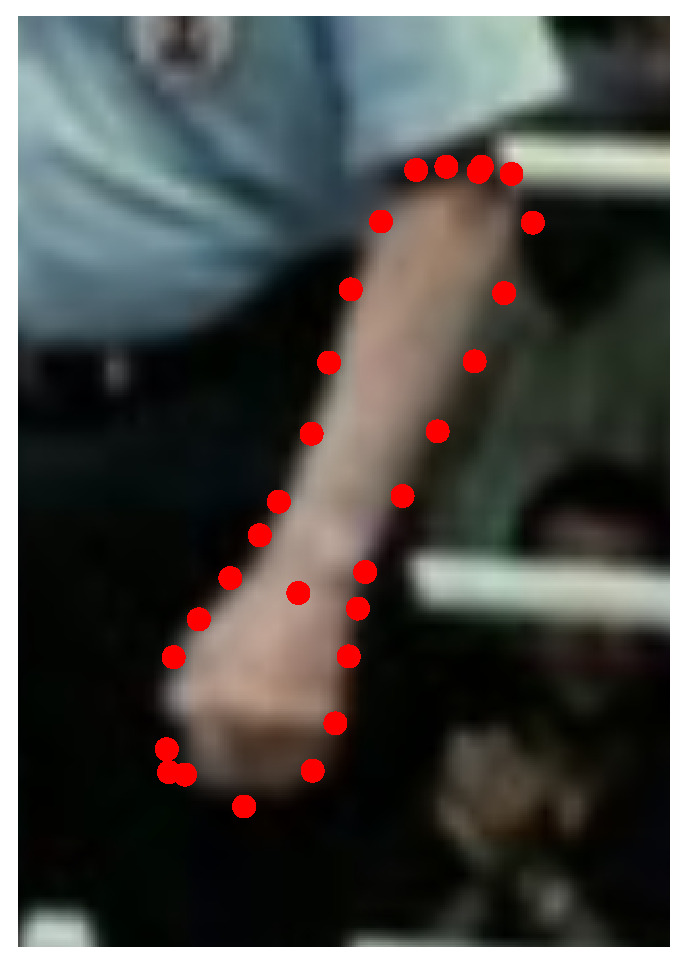
\includegraphics[height=\ofh]{resources/Fittings/27.eps}
    \hfill
    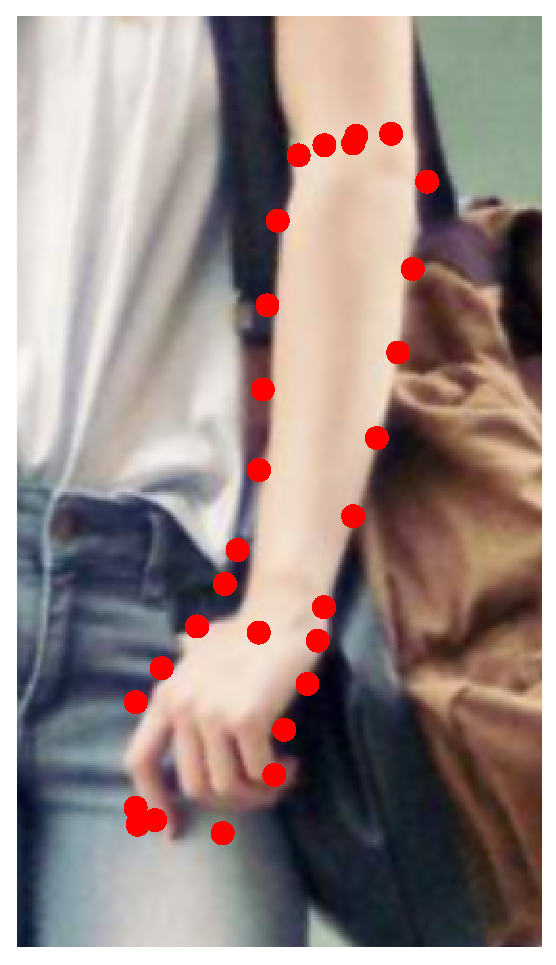
\includegraphics[height=\ofh]{resources/Fittings/29.eps}
    \hfill
    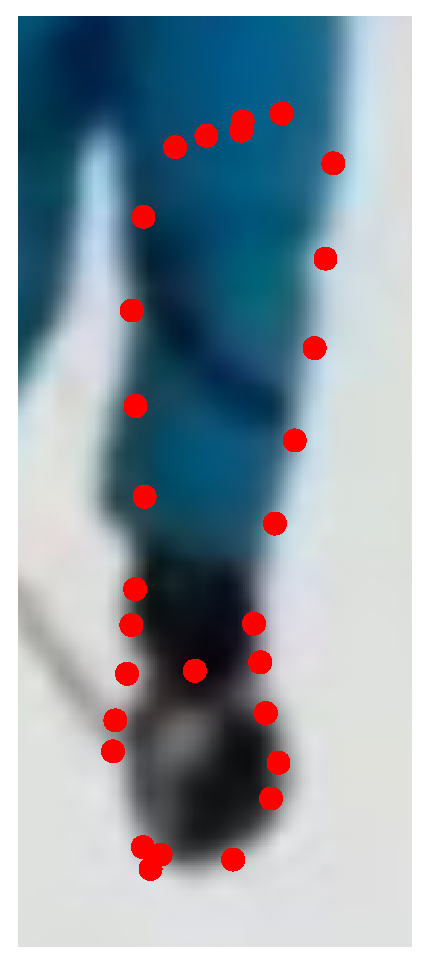
\includegraphics[height=\ofh]{resources/Fittings/31.eps}
    \hfill
    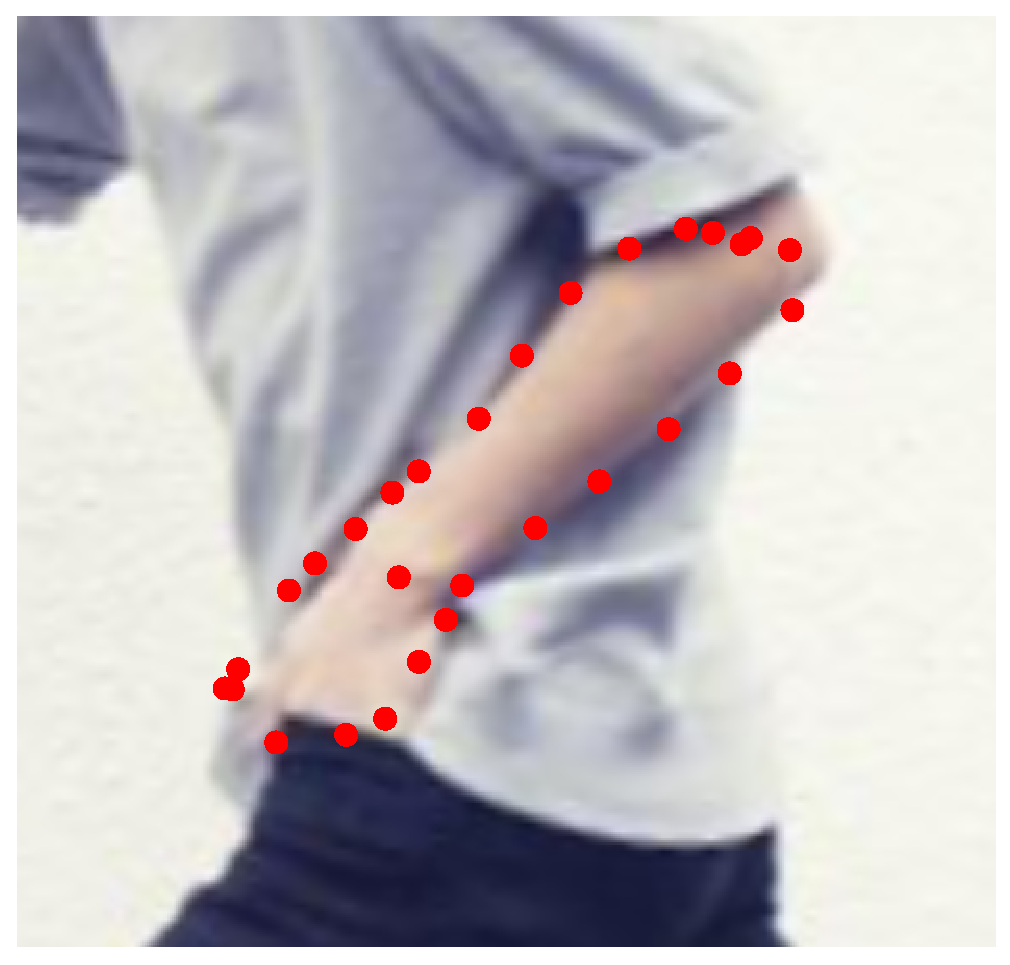
\includegraphics[height=\ofh]{resources/Fittings/33.eps}
    \hfill
    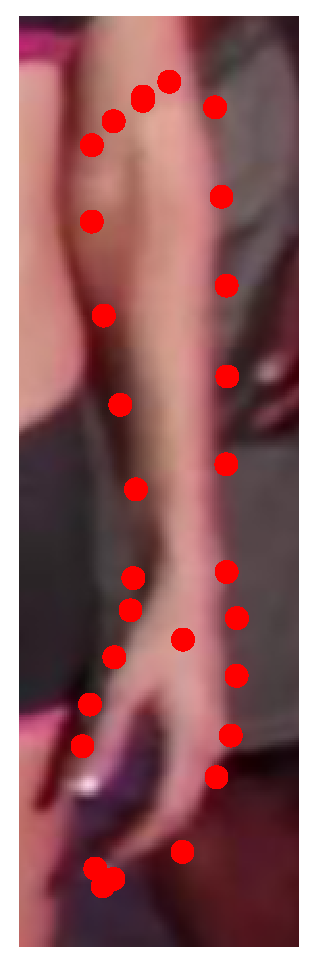
\includegraphics[height=\ofh]{resources/Fittings/35.eps}
    \hfill
    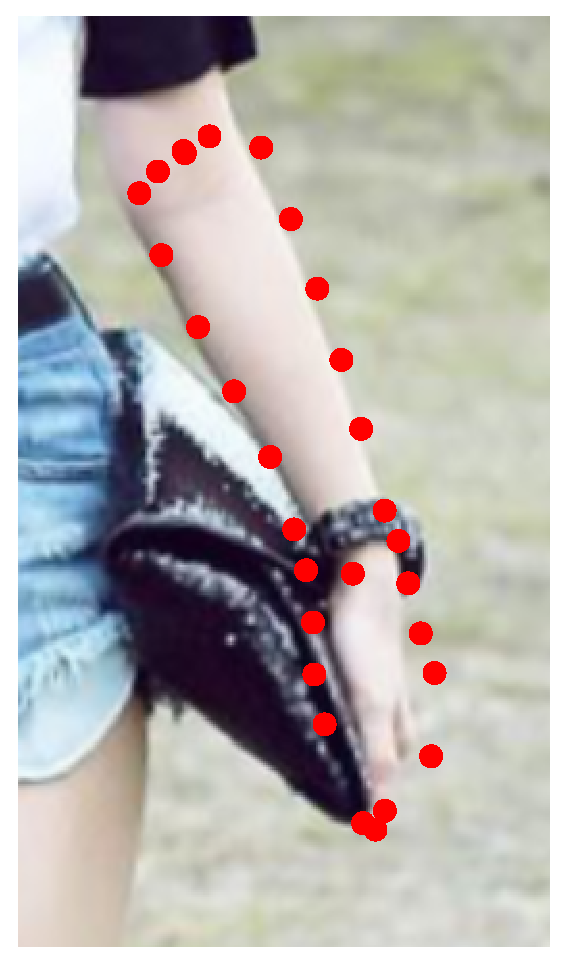
\includegraphics[height=\ofh]{resources/Fittings/36.eps}
    \hfill
    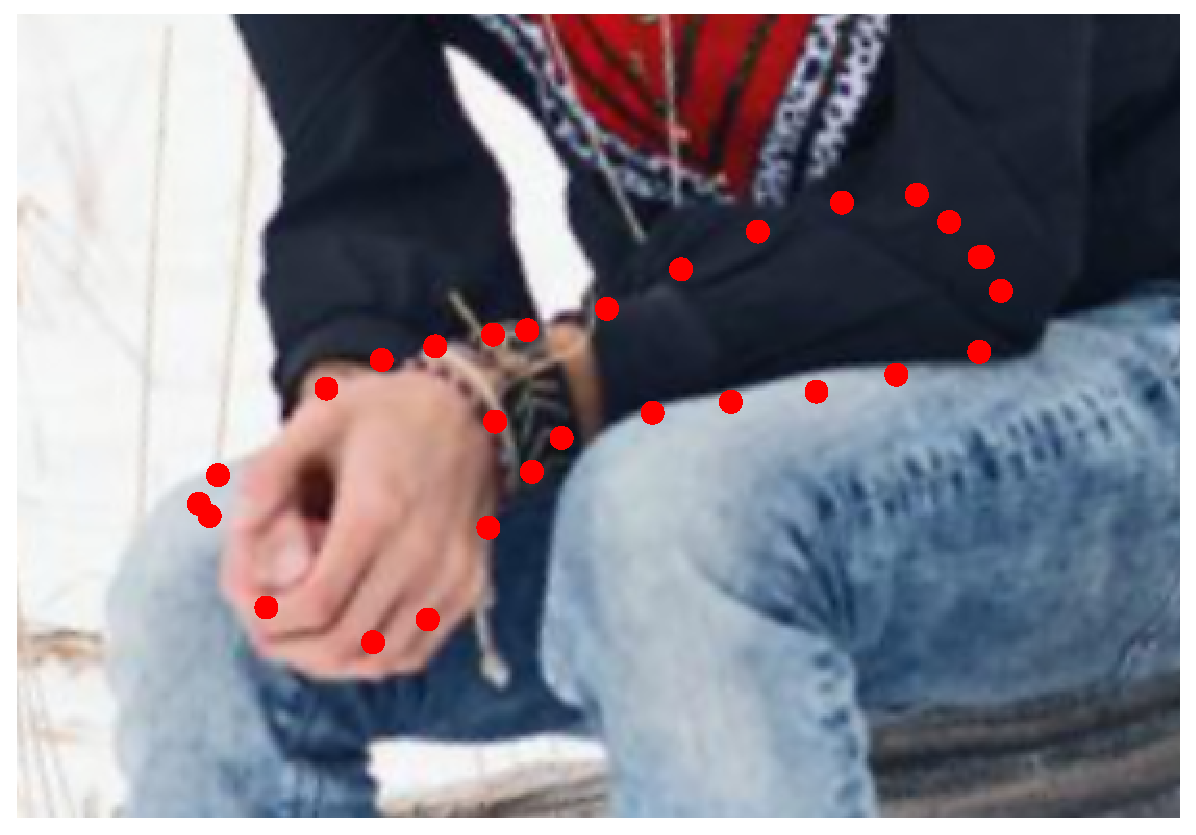
\includegraphics[height=\ofh]{resources/Fittings/37.eps}
    \hfill
    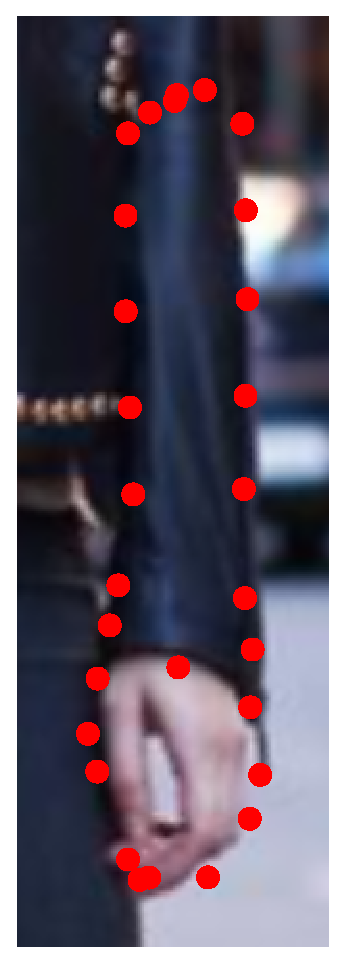
\includegraphics[height=\ofh]{resources/Fittings/38.eps}
    \hfill
    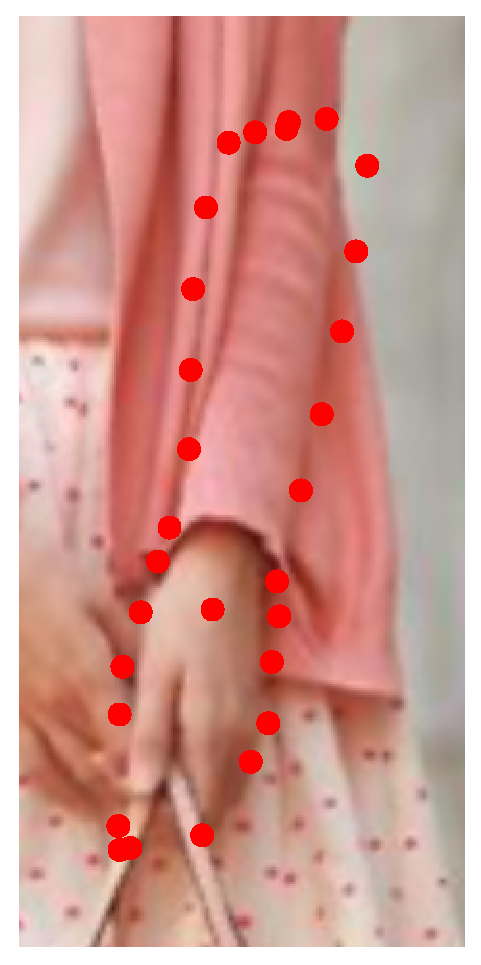
\includegraphics[height=\ofh]{resources/Fittings/39.eps}
    \caption{Demonstration of outline fitting of patch-based AAM on arms.}
    \label{fig:outline_fitting}
\end{figure*}




\subsection{Non-rigid Object Alignment In-the-wild}
\label{exp:daam_benchmark}
Herein, we compare the fitting accuracy of the dAAMs that are trained with our proposed framework with holistic sparse AAMs~\cite{Cootes2001,Matthews2004}. We consider two object classes that demonstrate rich texture: face and ear.

\noindent\textbf{Databases \& Error Metrics} In the case of face, we build both models using the 811 training images of the Labelled Faces Parts in-the-Wild (LFPW) \cite{belhumeur2013localizing}. Sparse AAMs were built from the 68 points annotations provided by~\cite{sagonas_iccv_300w_2013}. Our dAAMs were built as described in Step~\ref{sec:step4}. In both cases we build the appearance models using pixel intensities. The results are reported on the 224 images of the LFPW testset. The fitting error is evaluated as the point-to-point distance normalised by the face's size.

In the case of the ear, given the lack of publicly available annotated databases, we collected 605 high resolution images from the internet, that were captured under unconstrained conditions. The images were manually annotated with respect to a 55 point sparse annotation mark-up, as well as the curve annotations proposed in this paper. Examples of these two type of ear annotations are shown in Figure \ref{fig:intro}. We randomly split the database into two disjoint sets of training (500) and testing (105) images. The training and evaluation of the two models is done in the same way as in the face's case.

\begin{figure}[b!]
    \centering
    \includegraphics[width=0.6\columnwidth]{resources/DAAMBenchmark/legend}
    \\
    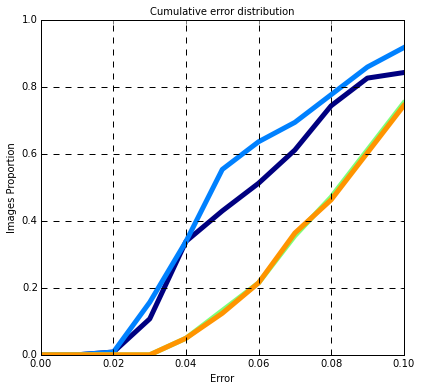
\includegraphics[width=0.48\columnwidth]{resources/DAAMBenchmark/face}
    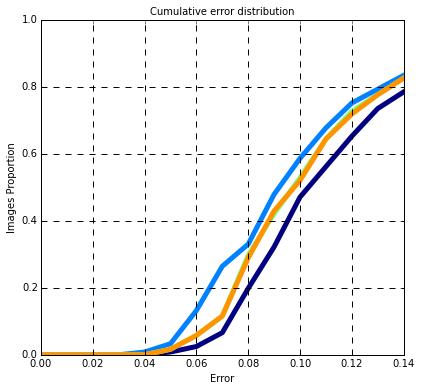
\includegraphics[width=0.48\columnwidth]{resources/DAAMBenchmark/ear}
    \caption{CEDs of faces and ears fitting performance for experiment \ref{exp:daam_benchmark}}
    \label{fig:daam_benchmark}
\end{figure}

\noindent\textbf{Results} We report the results in Figure \ref{fig:daam_benchmark} using Cumulative Error Distribution (CED) curves. By visually inspecting the results, we determined that the fitting is becomes inaccurate for errors greater than 0.1 and 0.06 for the ear and face, respectively. By inspecting the error curves, it can be observed that dAAMs marginally outperform sparse AAMs using pixels intensities as features. Therefore, the proposed pipeline is capable of dealing with the complex structure of non-rigid shapes and learn dAAMs from simple curve line annotations that can compete and even surpass the commonly-used sparse AAMs.


\subsection{Arm Pose Estimation}
\label{exp:benchmark}

In this experiment, we aim to compare the performance of a deformable model for the outline of the arm that is built on our proposed outline sparse annotation scheme, against the standard skeleton joints scheme that is commonly employed in literature. For this purpose, we employ the patch-based AAM as described in Step~\ref{sec:step4} and train two different models, one that corresponds to the outline of the arm and one on the skeleton of the hand.  Additionally, we compare are methodology with the current state-of-the-art techniques on human arm pose estimation in-the-wild.


\begin{figure}[b!]
    \centering
    \includegraphics[width=\columnwidth]{resources/HandBenchmark/legend}
    \\
    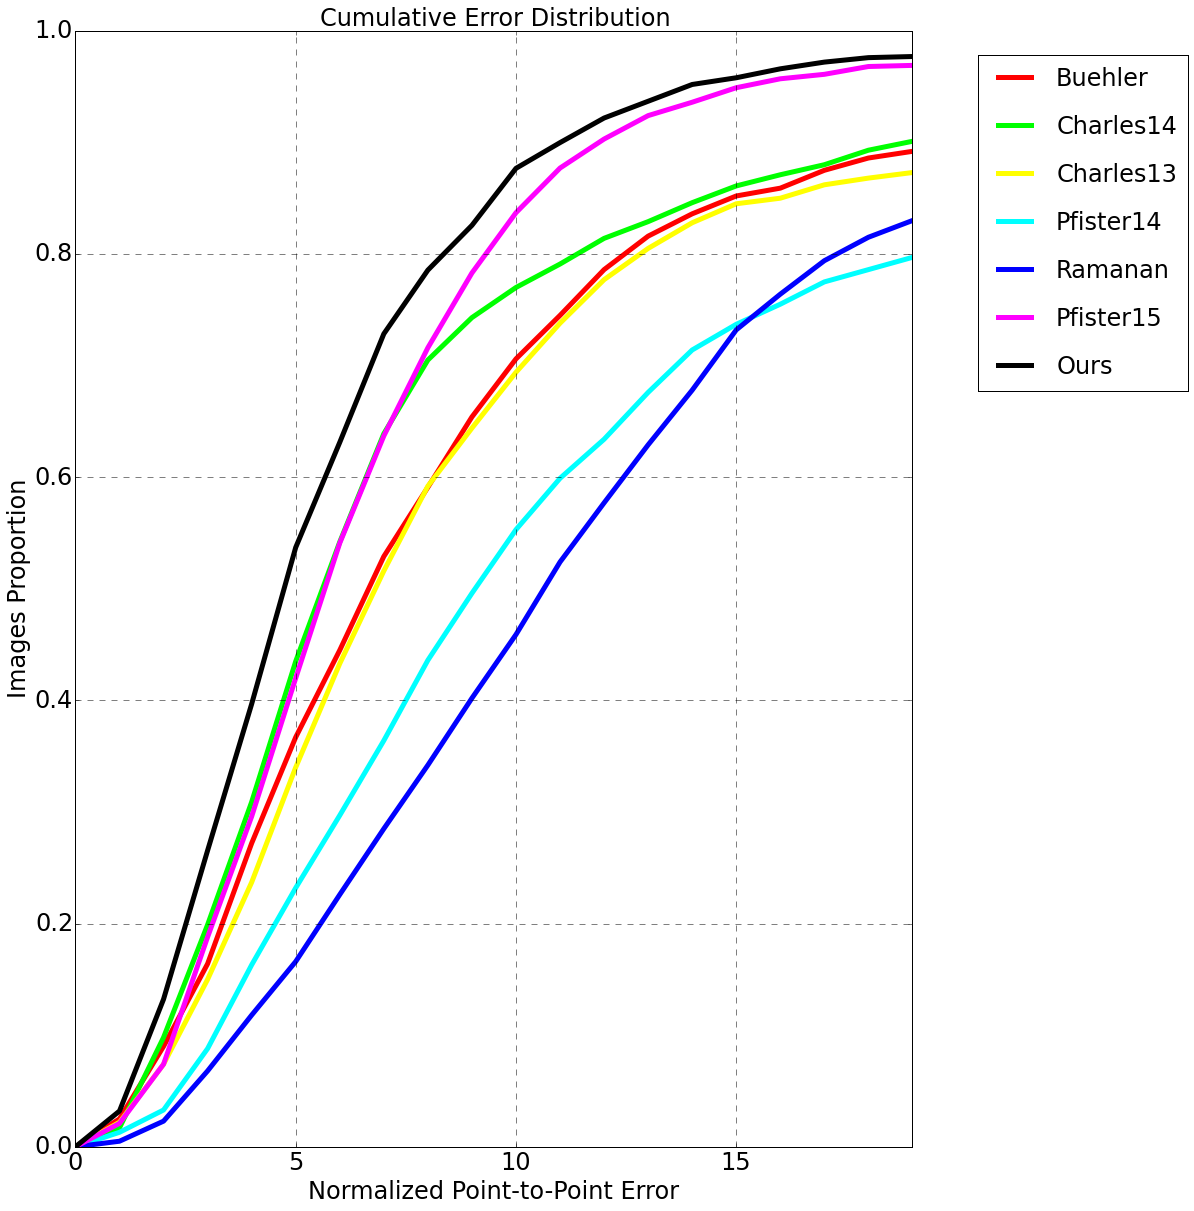
\includegraphics[width=0.48\columnwidth]{resources/HandBenchmark/wrist}
    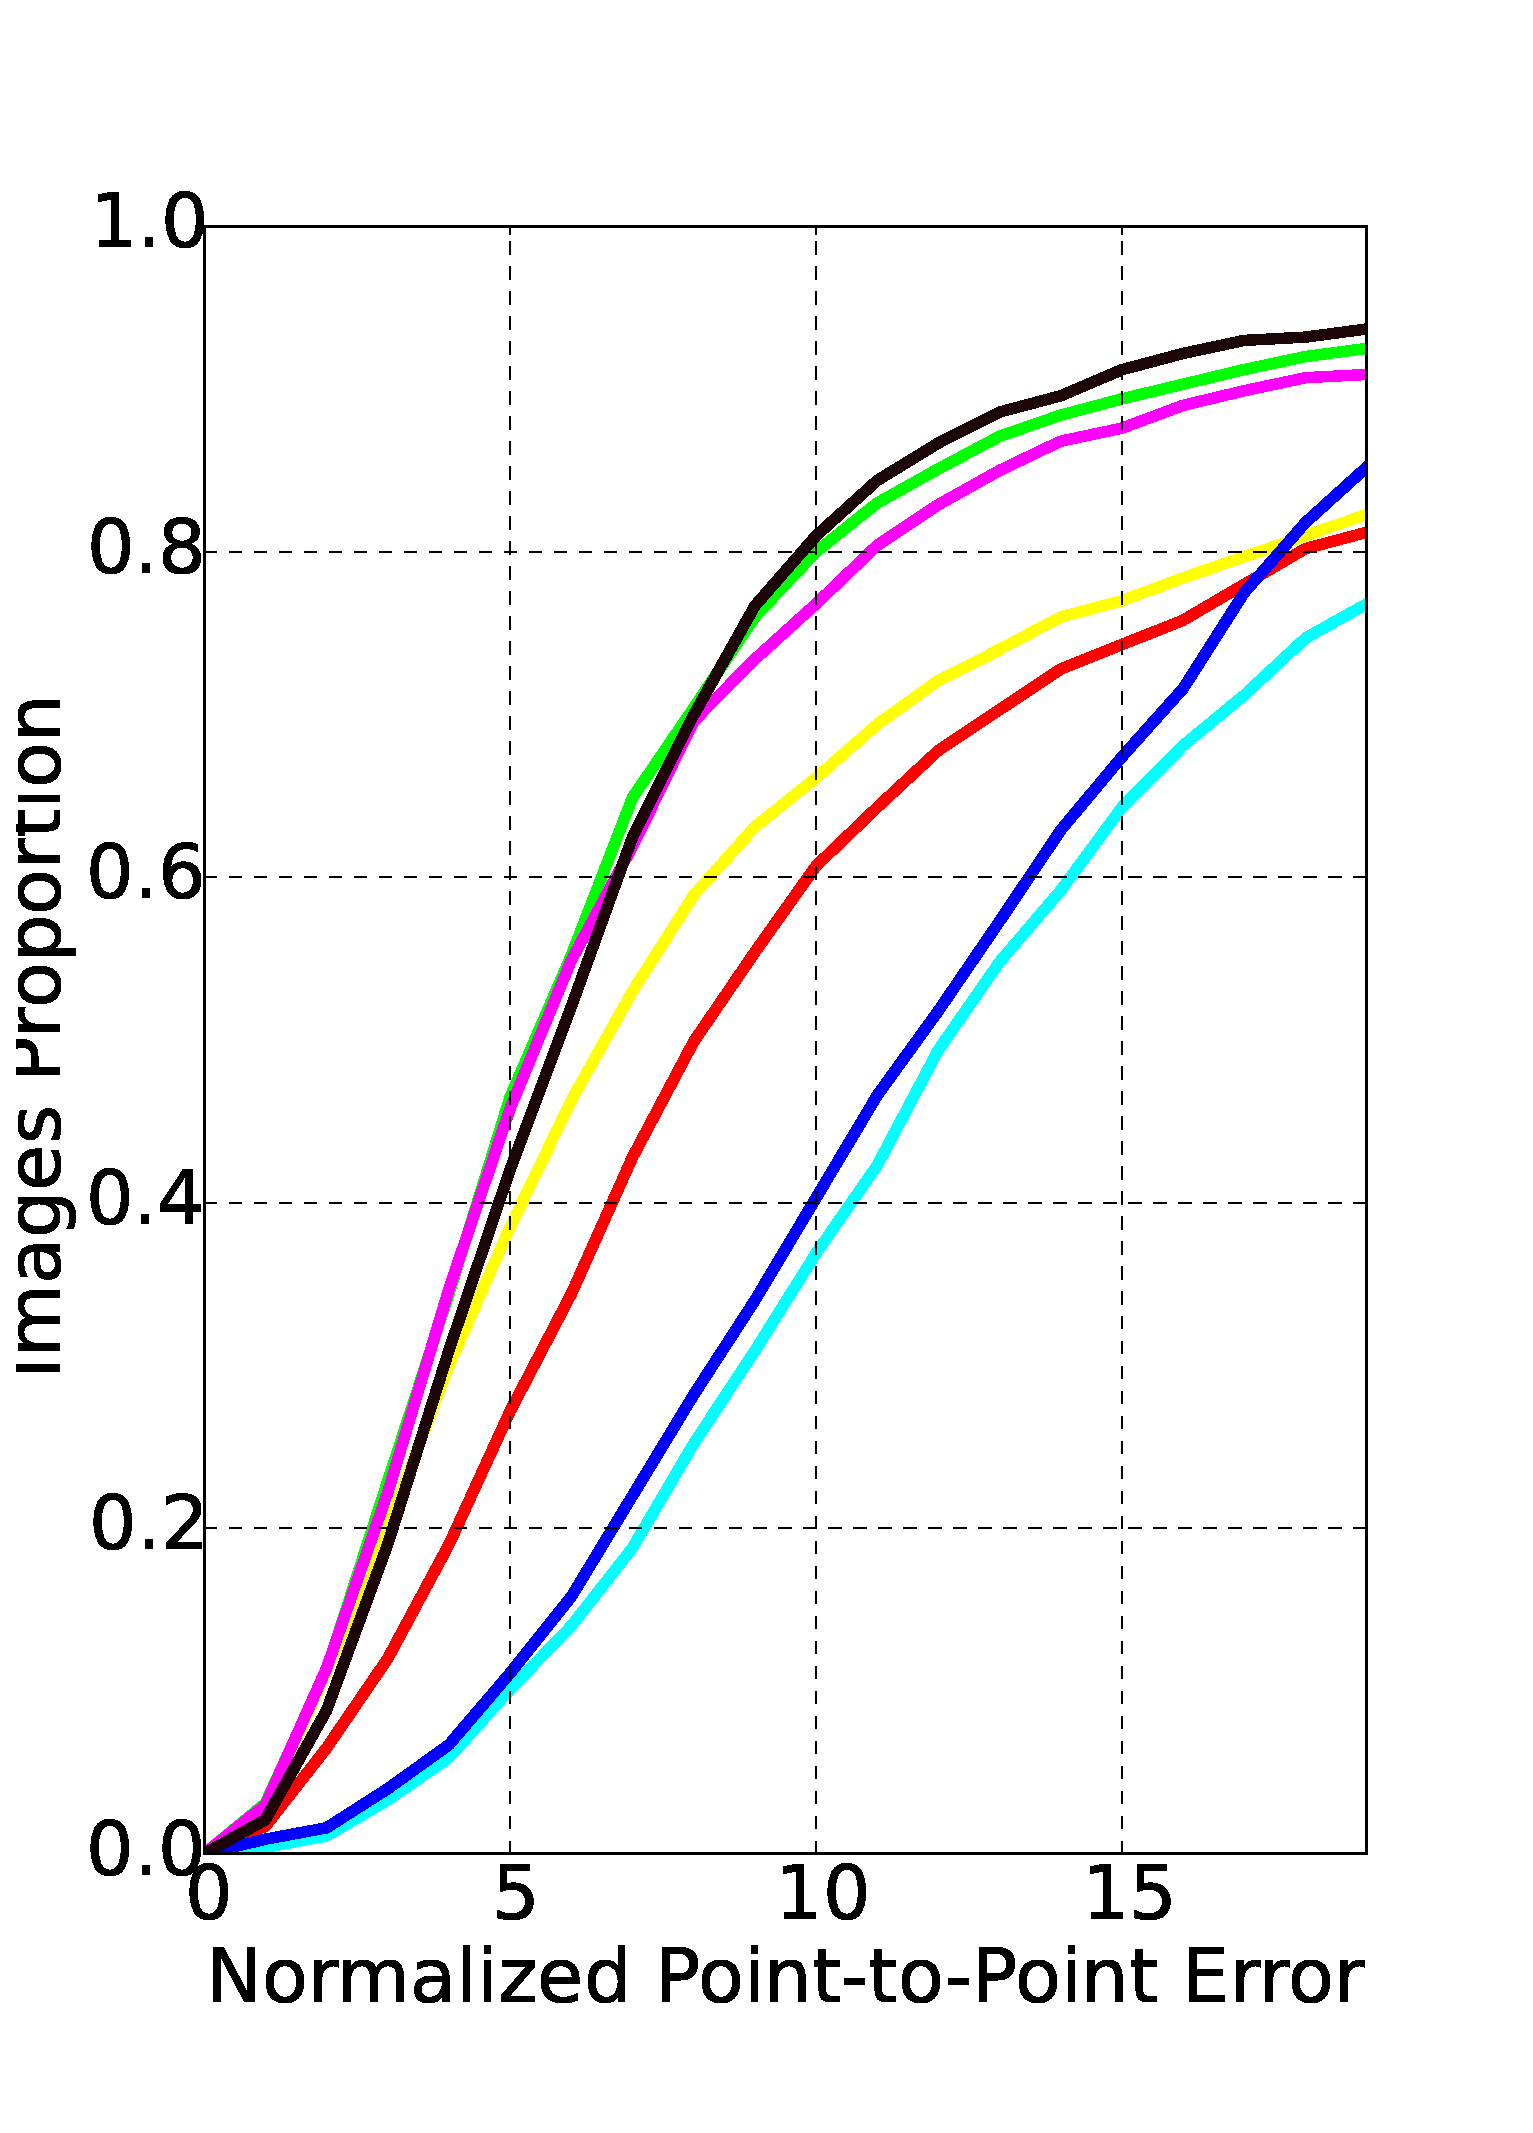
\includegraphics[width=0.48\columnwidth]{resources/HandBenchmark/elbow}
    \caption{CEDs over skeleton landmarks on BBC Pose database for experiment \ref{exp:benchmark}}
    \label{fig:hand_benchmark}
\end{figure}


\noindent\textbf{Dataset \& Error Metric} We opted to report quantitative results on the BBC Pose\cite{pfister2015flowing} database, which contains the most consistent skeleton annotations among all the existing ones. The training of the outline patch-based AAM was performed after obtaining the outline annotations using our proposed framework. To train the part-based AAM (29 landmarks in the boundary) we used 891 training images from a combination of datasets, including H3D \cite{PoseletsICCV09}, Microsoft COCO \cite{lin2014microsoft}, MPII \cite{andriluka14cvpr}, Fashion Pose \cite{dantone2013human}, FLIC \cite{sapp2013modec} and BBC Poses \cite{pfister2015flowing}. SIFT \cite{PoseletsICCV09} feature is used from image representation for our model. Model fitting on BBC Pose is initialised based on an in house deep convolutional neural network.

In order to compare with current state-of-the-art human pose estimation on BBC Pose, we used the same error metric as BBC Pose, which normalises testing images to have height of 256 pixels. Performance measure of experiments in this paper are plot with Cumulative Error Distribution (CED) curve, where graph shows accuracy against distance from ground truth in pixels on normalised images. Results for this experiment are reported over 1000 testing images BBC Pose Provided, which human upper-body pose are landmark with 7 points on skeleton. For our model, joints are projected from the dense correspondence generated from our proposed method. Results (Figure \ref{fig:hand_benchmark}, our method is the outline PAAM) are reported comparing with the state-of-the-art which includes Buehler \cite{buehler2011upper}, Charles14 \cite{charles2014upper}, Charles13 \cite{charles2013domain}, Pfister14 \cite{pfister2015deep}, Ramanan \cite{yang2013articulated} and Pfister15 \cite{pfister2015flowing}. As can seen our outline part-based AAM model, even though not trained for locating the wrist and elbow, outperforms the state-of-the-art for this task. In particular, our method improves performance of current best method \cite{pfister2015flowing} by a notable amount (9\% with error less than 6pt) on wrist, as well as marginal improvement on elbow estimation.

In the same experiment we investigated the disadvantages of using skeleton annotation. We build patch-based AAM on the skeleton of the arm with same training data. As it can be seen from the  CED curves of \ref{fig:hand_benchmark} the skeleton based deformable model (called joint PAAM) has significant lower performance than the our outline model (Outline PAAM),


% \begin{figure*}[!t]
%     \newcommand{\fh}{0.24\columnwidth}
%     \centering
%     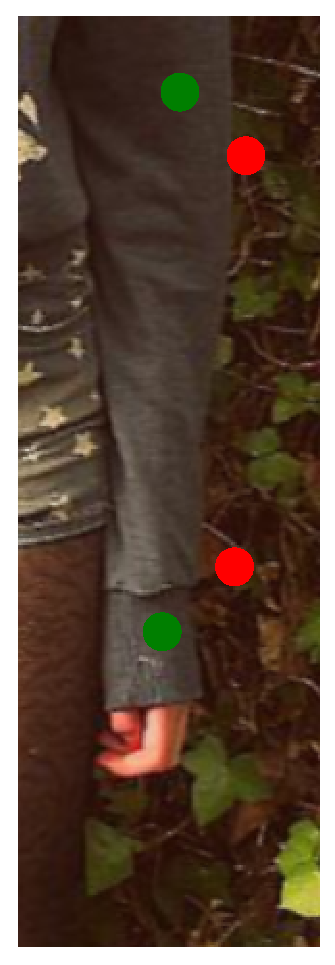
\includegraphics[height=\fh]{resources/Fixing/fix_1}
%     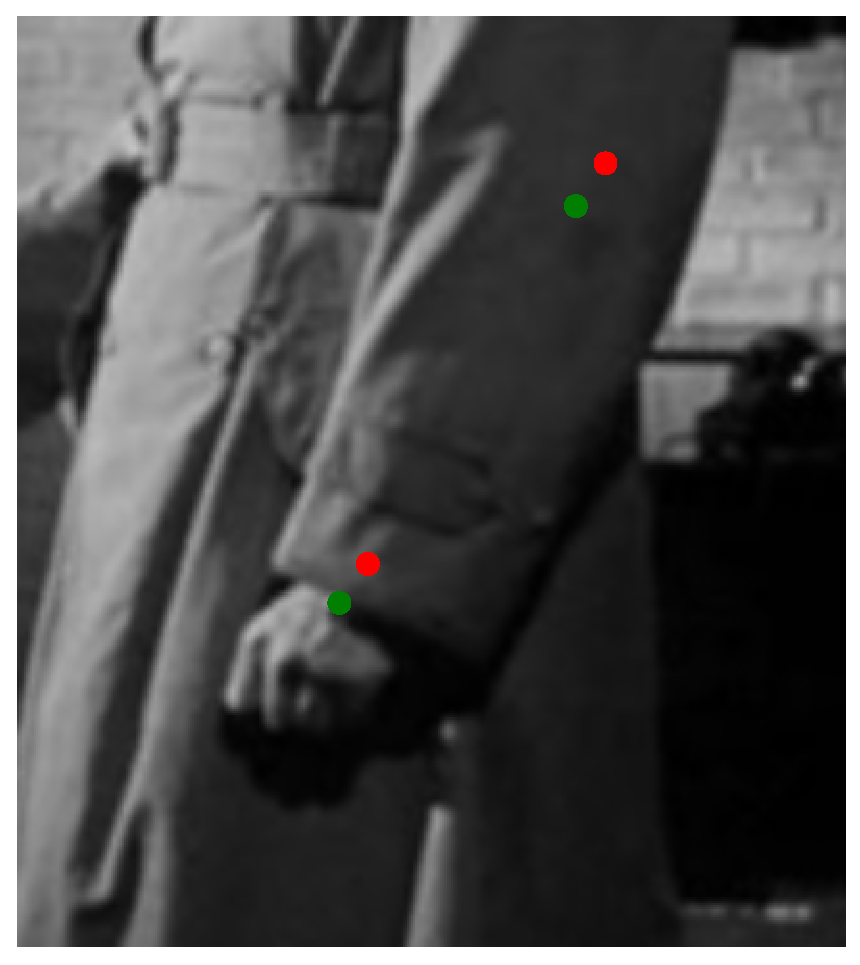
\includegraphics[height=\fh]{resources/Fixing/fix_2}
%     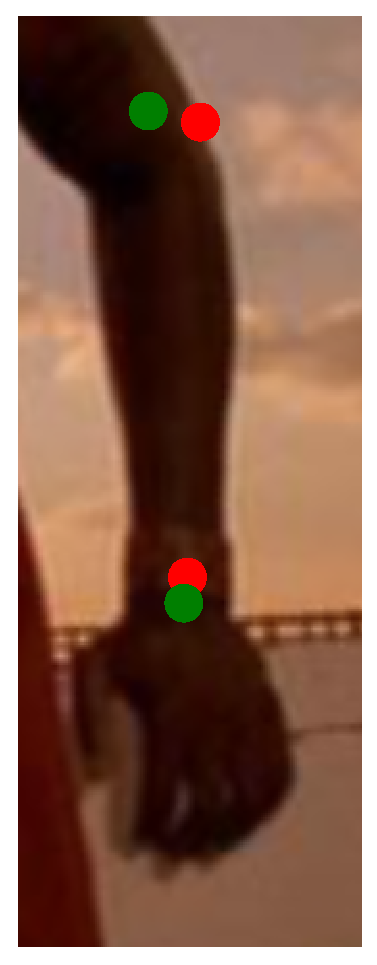
\includegraphics[height=\fh]{resources/Fixing/fix_3}
%     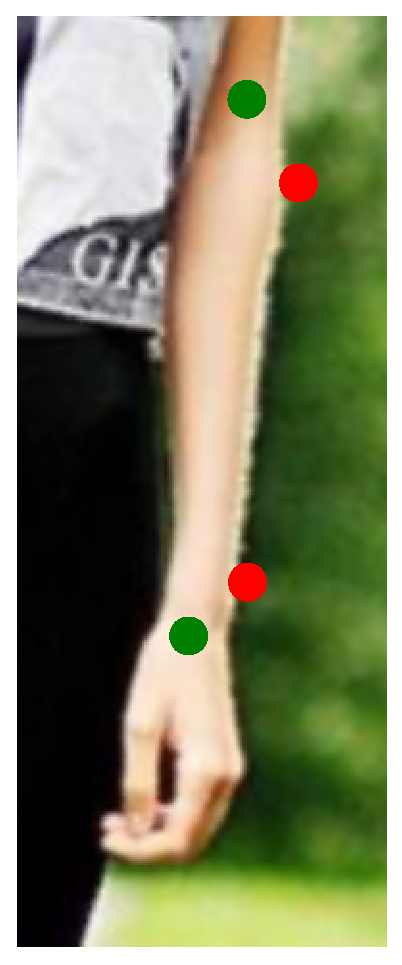
\includegraphics[height=\fh]{resources/Fixing/fix_5}
%     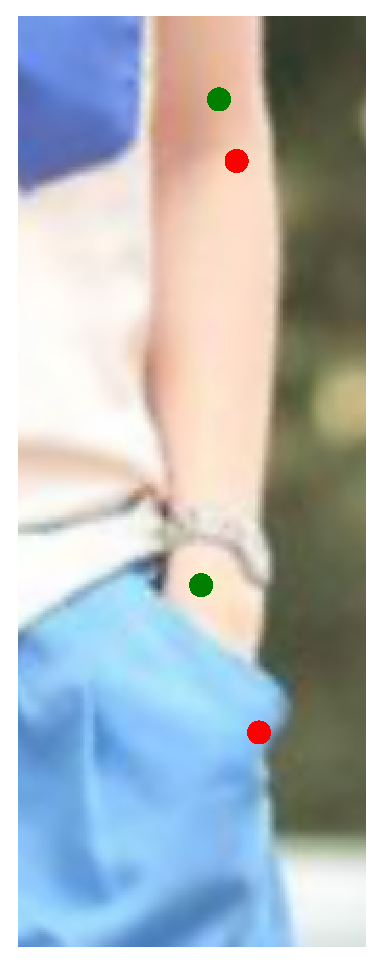
\includegraphics[height=\fh]{resources/Fixing/fix_6}
%     \includegraphics[height=\fh]{resources/Fixing/fix_7}
%     \includegraphics[height=\fh]{resources/Fixing/fix_8}
%     \includegraphics[height=\fh]{resources/Fixing/fix_9}
%     \includegraphics[height=\fh]{resources/Fixing/fix_10}
%     \includegraphics[height=\fh]{resources/Fixing/fix_20}
%     \includegraphics[height=\fh]{resources/Fixing/fix_12}
%     \includegraphics[height=\fh]{resources/Fixing/fix_13}
%     \includegraphics[height=\fh]{resources/Fixing/fix_14}
%     \includegraphics[height=\fh]{resources/Fixing/fix_15}
%     \includegraphics[height=\fh]{resources/Fixing/fix_17}
%     \includegraphics[height=\fh]{resources/Fixing/fix_18}
%     \caption{Demonstration of annotation correction using our method for experiment \ref{exp:qualitative}. \emph{Red} dots refer to officially provided landmarks, and \emph{green} dots are corrected position.}
%     \label{fig:qualitative}
% \end{figure*}

% \begin{figure*}[!t]
%     \newcommand{\ofh}{0.24\columnwidth}
%     \centering
%     \includegraphics[height=\ofh]{resources/Fittings/20.eps}
%     \includegraphics[height=\ofh]{resources/Fittings/3.eps}
%     \includegraphics[height=\ofh]{resources/Fittings/19.eps}
%     \includegraphics[height=\ofh]{resources/Fittings/4.eps}
%     \includegraphics[height=\ofh]{resources/Fittings/6.eps}
%     \includegraphics[height=\ofh]{resources/Fittings/15.eps}
%     \includegraphics[height=\ofh]{resources/Fittings/7.eps}
%     \includegraphics[height=\ofh]{resources/Fittings/8.eps}
%     \includegraphics[height=\ofh]{resources/Fittings/13.eps}
%     \includegraphics[height=\ofh]{resources/Fittings/17.eps}
%     \\
%     \includegraphics[height=\ofh]{resources/Fittings/21.eps}
%     \includegraphics[height=\ofh]{resources/Fittings/23.eps}
%     \includegraphics[height=\ofh]{resources/Fittings/25.eps}
%     \includegraphics[height=\ofh]{resources/Fittings/27.eps}
%     \includegraphics[height=\ofh]{resources/Fittings/29.eps}
%     \includegraphics[height=\ofh]{resources/Fittings/31.eps}
%     \includegraphics[height=\ofh]{resources/Fittings/33.eps}
%     \includegraphics[height=\ofh]{resources/Fittings/35.eps}
%     \includegraphics[height=\ofh]{resources/Fittings/36.eps}
%     \includegraphics[height=\ofh]{resources/Fittings/37.eps}
%     \includegraphics[height=\ofh]{resources/Fittings/38.eps}
%     \includegraphics[height=\ofh]{resources/Fittings/39.eps}
%     \caption{Demonstration of outline fitting of patch-based AAM on arms.}
%     \label{fig:outline_fitting}
% \end{figure*}

\subsection{Annotation Correction}
\label{exp:qualitative}

The final experiment demonstrates that is feasible to use the proposed arm model in order to correct the annotations provided by the current datasets. As mentioned above there are inconsistencies in the joint annotations of MPII \cite{andriluka14cvpr}, Fashion Pose \cite{dantone2013human} and FLIC \cite{sapp2013modec}. Three well trained annotators are used to annotate left arm using 120 test images from Fashion Pose \cite{dantone2013human} dataset. Figure \ref{fig:variance} presents statistical results calculated using data annotated and officially provided with normalisation based on length of arms. Exemplar annotation visualisation also shows significant inconsistency of manual annotation on joints.

Figure \ref{exp:qualitative} presents corrections of joint annotations using the proposed patch-based SDM. \emph{Red} dots shows ``ground truth" annotations while \emph{green} dots shows landmarks after correction using our methodology. There is no doubt that points after correction show more consistency among images. Images are cropped to hand only for better visualisation. Upon acceptance we will provide the corrected annotations in all the aforementioned databases.


















% \begin{table}[b!]
%     \small
%     \centering
%     \begin{tabular}{|l|c|c|c||c|c|c|}
%         \hline
%                             & \multicolumn{3}{c||}{Wrist} & \multicolumn{3}{c|}{Elbow}\\
%         \hline
%         \emph{Method}       & \emph{mean} & \emph{std} & $\leq 6pt$ & \emph{mean} & \emph{std} & $\leq 6pt$\\
%         \hline\hline
%         Buehler             & 12.08    & 19.94        & 44.5\%       & 12.94    & 14.65        & 34.4\%\\
%         Charles14           & 11.81    & 20.89        & 54.2\%       &  8.30    & 11.00        & \textbf{55.2\%}\\
%         Charles13           & 13.78    & 22.39        & 43.3\%       & 13.17    & 18.74        & 46.3\%\\
%         Pfister14           & 14.69    & 17.89        & 29.7\%       & 14.60    & 10.59        & 14.0\%\\
%         Ramanan             & 15.59    & 19.04        & 22.6\%       & 15.53    & 10.82        & 15.8\%\\
%         Pfister15           & 7.62     & 11.04        & 54.1\%       &  8.84    & 11.44        & 54.9\%\\
%         \hline\hline
%         Ours                & \textbf{6.71}& \textbf{10.90}   & \textbf{63.1\%}       & \textbf{8.20}     &  \textbf{10.54}        & 52.1\%\\
%         \hline
%     \end{tabular}
%     \caption{Fitting statistics on BBC Pose database for experiment \ref{exp:benchmark}}
%     \label{tab:hand_benchmark}
